% XML-filerna är skapade med hjälp av draw.io. Använd https://www.draw.io/ för att redigera dessa.

\documentclass[a4paper,12pt]{article}
\usepackage{graphicx}
\usepackage[backend=biber]{biblatex}
\usepackage{float}
\usepackage[swedish]{babel}
\usepackage[titletoc]{appendix}
\usepackage{pdfpages}
\addbibresource{bibliography.bib}
%% Definitioner f�r LIPS-dokument

\usepackage[utf8]{inputenc}
\usepackage[swedish]{babel}
\usepackage[T1]{fontenc}
\usepackage{times}
\usepackage{ifthen}

\usepackage[margin=25mm]{geometry}

\usepackage{fancyhdr}
\pagestyle{fancy}
\lhead{}
\chead{\textbf{\LIPSprojekttitel}}
\rhead{\textbf{\LIPSdatum}}
\lfoot{\textbf{\LIPSkursnamn}\\\textbf{LIPS Teknisk Dokumentation}}
\cfoot{\textbf{\thepage}\\\textbf{\LIPSgruppepost}}
\rfoot{\textbf{\LIPSprojektgrupp}}

\setlength{\parindent}{0pt}
\setlength{\parskip}{1ex plus 0.5ex minus 0.2ex}


\newcommand{\twodigit}[1]{\ifthenelse{#1<10}{0}{}{#1}}
\newcommand{\dagensdatum}{\number\year-\twodigit{\number\month}-\twodigit{\number\day}}

%%  Redefinitions of commands containing @
\makeatletter
\makeatother

\newcommand{\LIPStitelsida}{%
{\ }\vspace{45mm}
\begin{center}
  \textbf{\Huge \LIPSdokumenttyp}
\end{center}
\begin{center}
  {\Large Redaktör: \LIPSredaktor}
\end{center}
\begin{center}
  {\Large \textbf{Version \LIPSversion}}
\end{center}
\begin{center}
  {\LIPSBeskrivning}
\end{center}
\vfill
\begin{center}
  {\large Status}\\[1.5ex]
  \begin{tabular}{|*{3}{p{40mm}|}}
    \hline
    Granskad & \LIPSgranskare & \LIPSgranskatdatum \\
    \hline
    Godkänd & \LIPSgodkannare & \LIPSgodkantdatum \\
    \hline
  \end{tabular}
\end{center}
\newpage
}


\newenvironment{LIPSprojektidentitet}{%
{\ }\vspace{45mm}
\begin{center}
  {\Large PROJEKTIDENTITET}\\[0.5ex]
  {\small
  \LIPSartaltermin, \LIPSprojektgrupp\\
  Linköpings Tekniska Högskola, IFM
  }
\end{center}
\begin{center}
  {\small Gruppdeltagare}\\
%  \begin{tabular}{|p{30mm}|p{40mm}|p{35mm}|p{45mm}|}
  \begin{tabular}{|l|l|p{25mm}|l|}
    \hline
    \textbf{Namn} & \textbf{Ansvar} & \textbf{Telefon} & \textbf{E-post} \\
    \hline
}%
{%
    \hline
  \end{tabular}
\end{center}
\begin{center}
  {\small
    %\textbf{E-postlista för hela gruppen}: \LIPSgruppepost\\
    %\textbf{Hemsida}: \LIPSgrupphemsida\\[1ex]
    \textbf{Kund}: \LIPSkund\\
    \textbf{Kontaktperson hos kund}: \LIPSkundkontakt\\
    \textbf{Kursansvarig}: \LIPSkursansvarig\\
    \textbf{Handledare}: \LIPShandledare\\
  }
\end{center}
\newpage
}
\newcommand{\LIPSgruppmedlem}[4]{\hline {#1} & {#2} & {#3} & {#4} \\}



\newenvironment{LIPSdokumenthistorik}{%
\begin{center}
  Dokumenthistorik\\[1ex]
  \begin{small}
    \begin{tabular}{|l|l|p{60mm}|l|l|}
      \hline
      \textbf{Version} & \textbf{Datum} & \textbf{Utförda förändringar} & \textbf{Utförda av} & \textbf{Granskad} \\
      }%
    {%
      \hline
    \end{tabular}
  \end{small}
\end{center}
}

\newenvironment{LIPSlicens}{\begin{center}\large{Licens}\end{center}}{}
 
\newcommand{\LIPSversionsinfo}[5]{\hline {#1} & {#2} & {#3} & {#4} & {#5} \\}

\newcounter{LIPSkravnummer}
\newcounter{LIPSunderkravnummer}[LIPSkravnummer]
\newenvironment{LIPSkravlista}{%
  \begin{tabular}{|p{25mm}|p{25mm}|p{72mm}|p{18mm}|}
    }%
  {%
    \hline
  \end{tabular}
}
\newcommand{\LIPSkrav}[3]{\hline\stepcounter{LIPSkravnummer}\textbf{Krav nr \arabic{LIPSkravnummer}} & \textbf{{#1}} & {#2} & \textbf{{#3}} \\}
\newcommand{\LIPSunderkrav}[3]{\hline\stepcounter{LIPSunderkravnummer}\textbf{Krav nr \arabic{LIPSkravnummer}\Alph{LIPSunderkravnummer}} & \textbf{{#1}} & {#2} & \textbf{{#3}} \\}

\newcounter{LIPSMilstolpar}
\newenvironment{LIPSMilstolpslista}{%
  \begin{tabular}{|p{15mm}|p{72mm}|p{25mm}|}
\hline
\textbf{Nr} & \textbf{Beskrivning} & \textbf{Datum} \\
    }%
  {%
  \hline
  \end{tabular}
}
\newcommand{\LIPSMilstolpar}[2]{\hline\stepcounter{LIPSMilstolpar}\textbf{ \arabic{LIPSMilstolpar}.} & \textbf{{#1}} & \textbf{{#2}} \\}

\newcounter{LIPSBeslutspunkter}
\newenvironment{LIPSBeslutspunktslista}{%
  \begin{tabular}{|p{15mm}|p{72mm}|p{25mm}|}
\hline
\textbf{Nr} & \textbf{Beskrivning} & \textbf{Datum} \\
    }%
  {%
  \hline
  \end{tabular}
}
\setcounter{LIPSBeslutspunkter}{-1}
\newcommand{\LIPSBeslutspunkter}[2]{\hline\stepcounter{LIPSBeslutspunkter}\textbf{ \arabic{LIPSBeslutspunkter}.} & \textbf{{#1}} & \textbf{{#2}} \\}

\newcounter{LIPSAktiviteter}
\newenvironment{LIPSAktivitetslista}{%
  \begin{tabular}{|p{15mm}|p{72mm}|p{25mm}|}
\hline
\textbf{Nr} & \textbf{Beskrivning} & \textbf{Datum} \\
    }%
  {%
  \hline
  \end{tabular}
}
\newcommand{\LIPSAktiviteter}[2]{\hline\stepcounter{LIPSAktiviteter}\textbf{ \arabic{LIPSAktiviteter}.} & \textbf{{#1}} & \textbf{{#2}} \\}




%%% Local Variables: 
%%% mode: latex
%%% TeX-master: "kravspec_mall"
%%% End: 
\pagenumbering{roman}
\newcommand{\LIPSartaltermin}{2018/VT}
\newcommand{\LIPSkursnamn}{TFYA75}

\newcommand{\LIPSprojekttitel}{Visualisering av elektronstruktur}

\newcommand{\LIPSprojektgrupp}{Grupp 2}
\newcommand{\LIPSgruppepost}{}
\newcommand{\LIPSdokumentansvarig}{Marian Brännvall}

\newcommand{\LIPSkund}{IFM, Linköpings universitet, 581\,83 Linköping}
\newcommand{\LIPSkundkontakt}{Rickard Armiento, 013-281249, rickard.armiento@liu.se}
\newcommand{\LIPSkursansvarig}{Per Sandström, 013-282902, persa@ifm.liu.se}
\newcommand{\LIPShandledare}{Johan Jönsson, 013-281176, johan.jonsson@liu.se}


\newcommand{\LIPSdokumenttyp}{Teknisk dokumentation}
\newcommand{\LIPSredaktor}{Anders Rehult}
\newcommand{\LIPSversion}{1.0}
\newcommand{\LIPSBeskrivning}{Denna tekniska dokumentation är baserad på 2017 års tekniska dokumentation för visualiseringsvertyget ENVISIoN, se bilaga \ref{appendix:tekdok-2017}.}
\newcommand{\LIPSdatum}{\dagensdatum}

\newcommand{\LIPSgranskare}{PL}
\newcommand{\LIPSgranskatdatum}{2018-05-25}
\newcommand{\LIPSgodkannare}{Rickard Armiento}
\newcommand{\LIPSgodkantdatum}{2018-05-28}

\usepackage[titletoc]{appendix}
\usepackage{hyperref}
\hypersetup{
    colorlinks,
    citecolor=black,
    filecolor=black,
    linkcolor=black,
    urlcolor=black
}

\begin{document}

\LIPStitelsida

\begin{LIPSprojektidentitet}
  \LIPSgruppmedlem{Anders Rehult}{Projektledare (PL)}{076-3161206}{andre449@student.liu.se}
  \LIPSgruppmedlem{\LIPSdokumentansvarig}{Dokumentansvarig (DOK)}{070-7280044}{marbr639@student.liu.se}
  \LIPSgruppmedlem{Andreas Kempe}{Sekreterare (SE)}{073-9796689}{andke133@student.liu.se}
  \LIPSgruppmedlem{Viktor Bernholtz}{Viktor Bernholtz (VB)}{073-0386030}{vikbe253@student.liu.se}
\end{LIPSprojektidentitet}

\tableofcontents{}
\newpage

\addcontentsline{toc}{section}{Dokumenthistorik}
\begin{LIPSdokumenthistorik}
  \LIPSversionsinfo{0.1}{2018-05-18}{Första utkast.}{Projektgruppen}{PL}
  \LIPSversionsinfo{0.2}{2018-05-25}{Andra utkast (figur 11 uppdaterad).}{Projektgruppen}{PL}
    \LIPSversionsinfo{1.0}{2018-05-28}{Godkänd}{Projektgruppen}{PL}
  
\end{LIPSdokumenthistorik}

\newpage
\addcontentsline{toc}{section}{Licens}
\begin{LIPSlicens}
  2018 års modifikationer av den tekniska dokumentationen är licensierade under CC0, se bilaga~\ref{ref:licens}. 
 
\end{LIPSlicens}


\newpage
\pagenumbering{arabic}

\section{Inledning}
Dokumentet är en teknisk dokumentation för kandidatprojektet i visualisering av elektronstrukturer. Visualisering av elektronstrukturer är ett av projekten i kursen TFYA75 vid
Linköpings universitet. Den tekniska dokumentationen beskriver detaljerat hur systemet är implementerat.

\subsection{Parter}
Rickard Armiento har beställt systemet som är beskrivet i denna tekniska dokumentation. Medlemmarna i projektgruppen, som är listade under rubriken projektidentitet ovan, är mottagare av denna beställning och har haft i uppgift att implementera systemet. Projektgruppens handledare är Johan Jönsson.

\subsection{Syfte och mål}
Inom materialfysik är elektronstrukturberäkningar ett viktigt teoretiskt verktyg. Detta för att få en så bra förståelse som möjligt av hur olika material är uppbyggda, bland annat vad gäller kristallers egenskaper sett ur ett kvantmekaniskt perspektiv. Det kan exempelvis handla om att man vill ta reda på olika materials egenskaper vad gäller värmeledningsförmåga, strömledningsförmåga etc.

För att öka förståelsen samt för att enklare kunna presentera resultat från forskning inom området är det viktigt att kunna göra olika typer av visualiseringar baserat på elektronstrukturberäkningar.

I många av de system som används för att utföra dessa beräkningar, exempelvis VASP, ges ingen eller begränsad möjlighet till detta. Vidare är de system som idag finns tillgängliga för visualisering förhållandevis ineffektiva, dåligt standardiserade samt har få visualiseringsfunktioner.

Syftet och målet för projektet har varit att uppdatera och utöka det modifierbara verktyg för visualisering av resultaten från elektronstrukturberäkningar som togs fram av 2017 års projektgrupp. Utöver det konkreta målet med utvecklingen av mjukvara för visualisering ska även projektet ge projektmedlemmarna erfarenhet av att arbeta i projekt och utöka deras förmåga till analytiskt och fysikaliskt tänkande för att ge värdefull erfarenhet inför arbetslivet.

\subsection{Användning}
Denna produkt kommer användas vid Linköpings universitet för att analysera data från elektronstruktursberäkningar.

\subsection{Begränsningar}
I projektet kommer visualiseringsverktyget Inviwo och
programmeringspråken Python och C++ användas. Det kommer inte utredas
om det är bättre att använda andra verktyg.

\subsection{Definitioner}
\begin{itemize}
\setlength\itemsep{0em}
\item \textbf{Inviwo:} Ett forskningsverktyg som utvecklas vid Linköpings universitet och ger användaren möjlighet att styra visualisering med hjälp av programmering i Python 3 eller grafiskt. Det tillhandahåller även användargränssnitt för interaktiv visualisering.

\item \textbf{Processor:} Benämningen på ett funktionsblock i Inviwos nätverksredigerare som tar emot indata och producerar utdata. I detta dokument avser en processor alltid en inviwoprocessor om inte annat anges.

\item \textbf{Ports:} Kanaler som processorer använder för att utbyta data av specifika typer.

\item \textbf{MultiInports:} Ports som kan ta emot flera datastrukturer av samma typ.

\item \textbf{Properties:} Variabler som bestämmer en processors tillstånd.

\item \textbf{Länkar:} Kanaler som processorer använder för att länka samman properties av samma typ så att deras tillstånd synkroniseras.

\item \textbf{Inviwo-nätverk:} Ett antal processorer sammankopplade via portar och länkar.

\item \textbf{vec3:} Vektor med tre komponenter.

\item \textbf{Mesh:} Polygonyta.

\item \textbf{Volymdata:} Tredimensionella data.

\item \textbf{API} (Application Programming Interface): En specifikation av hur olika applikationer kan använda och kommunicera med en specifik programvara. Detta utgörs oftast av ett dynamiskt länkat bibliotek.
	\cite{API}

\item \textbf{BSD2} är en licens för öppen källkod.
	\cite{BSD2}

\item \textbf{C++} är ett programmeringsspråk.
	\cite{C++}
	\newline
	I Inviwo används C++ för att skriva programkod till processorer.

\item \textbf{Python} är ett programmeringsspråk.
	\cite{Python}
	\newline
	I Inviwo används Python för att knyta samman processorer.

\item \textbf{Fermi-energi} defineras som en energinivå där antalet tillstånd som har en energi lägre än Fermi-energin är lika med antalet elektroner i systemet. \cite{Fermi-energi}

\item \textbf{Fermi-yta} är, för elektroners k-punkter i reciproka rymden, isoytan där elektronernas energi är lika med Fermi-energin.
\cite{Fermi-yta}

\item \textbf{Git} är ett decentraliserat versionshanteringssystem.
\cite{Git}
    
\item \textbf{GUI} (Graphical User Interface) är ett grafiskt
användargränssnitt.
\cite{GUI}

\item \textbf{HDF5} är ett filformat som kan hantera stora mängder data \cite{hdf5}. Alla HDF5-objekt har en rotgrupp som äger alla andra objekt i datastrukturen. Denna grupp innehåller i sin tur all övrig data i form av andra grupper, länkar till andra grupper eller dataset. Dataset innehåller rådata av något slag. Rådata kan i sammanhanget vara bilder, utdata från beräkningar, programdata, etc. \cites[4-5]{hdf5-intro}

De övriga objektstyperna gås inte igenom i detalj i detta dokument,
men finns väl beskrivna i \emph{High Level Introduction to HDF5} \cite{hdf5-intro}.

\item \textbf{VASP} är ett program för modellering på atomnivå, för t.ex. elektronstruktusrberäkningar och kvantmekanisk molekyldynamik.
\cite{VASP}

\item \textbf{Rastergrafik} är en typ av data som innehåller en matris av färgvärden, med bestämd och informationsbegränsad upplösning.
\cite{raster}

\end{itemize}

\section{Produkten}
Visualiseringsverktyget kan visualisera elektrontäthet, ELF (Electron localization function), kristallstruktur som atompositioner i enehetscellen samt total och partiell tillståndstäthet.
% TODO: Lägg till Fermi om det lyckas visualiseras.

Figur \ref{fig:interface} visar vad användaren ser när ELF-data för diamant visualiseras. Längst till vänster i figuren ses ett fönster med Properties, i detta fall för processorn ELF raycasting som kan hittas i nätverket längst till höger i figuren. Properties för de olika processorerna fås när en processor är markerad. I mitten av figuren ligger den utritade bilden. Bilden kan roteras genom att klicka och dra i den. I fönstret Properties finns en Property vid namn Transfer function, med hjälp av vilken användaren kan ändra transparens/opacitet samt färg, se figur \ref{fig:transferfunction}.

\begin{figure}[H]
	\centering
	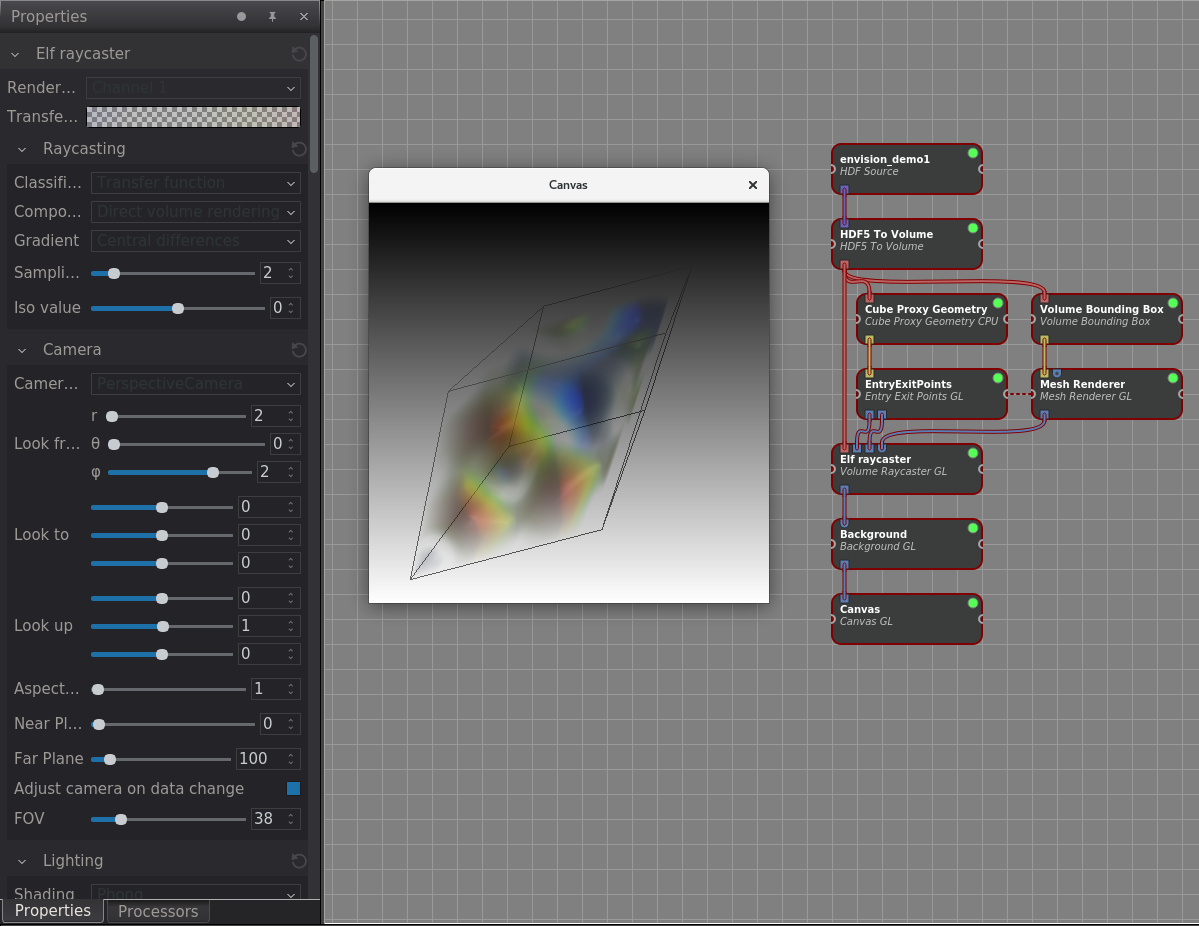
\includegraphics[scale=0.3]{inviwo_interface_elf.png}
	\caption{Bild av vad användaren ser när ELF visualiseras, i detta fall för diamant.}
	\label{fig:interface}
\end{figure}

\begin{figure}[H]
	\centering
	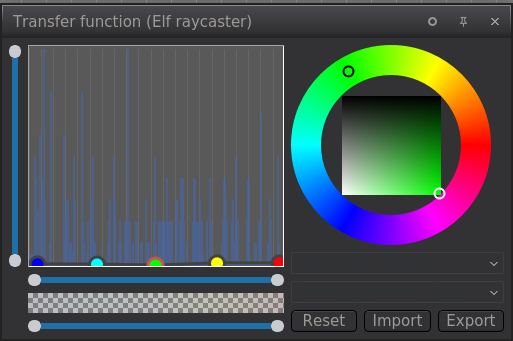
\includegraphics[scale=0.55]{transferfunction_elf.png}
	\caption{Transfer function property där transparens och färg kan ställlas in.}
	\label{fig:transferfunction}
\end{figure}

\section{Översikt av systemet}
Systemet är ett visualiseringsverktyg som kan användas för att visualisera utdata från elektronstrukturberäkningar i beräkningsprogrammet VASP. Programmet är modulärt programmerat och styrs via ett API.

\subsection{Resurser}
Följande resurser har använts för att utveckla systemet:

Mjukvara:
\begin{itemize}
\setlength\itemsep{0em}
\item Inviwo
\item h5py
\item Qt Creator
\item CMake
\item Git
\end{itemize}

Programmeringsspråk:
\begin{itemize}
\setlength\itemsep{0em}
\item Python 3
\item C++ 14
\end{itemize}

\subsection{Ingående delsystem}
\textbf{Delsystem 1 - System för parsning}
\newline Detta delsystem har i uppgift att läsa in data från VASP och omvandla till HDF5-format.

\textbf{Delsystem 2 - System för visualisering}
\newline Detta delsystem har i uppgift att visualisera data som parsats av delsystem 1.

\subsection{Utvecklingsfilosofi}
Projektet har drivits med hjälp av versionshanteringssystemet Git och koden är licensierad med BSD 2, men även utvecklad under Inviwos utvecklaravtal för att, om önskvärt, kunna officiellt integreras i programvaran.

\section{Delsystem 1 - System för parsning}
Delsystemet 1 för parsning består av ett pythonbibliotek av moduler för att kunna hantera de olika utdatafilerna från VASP. Varje modul används för att läsa in specifika data från varje enskild utdatafil. Systemet har också en modul som anropas av samtliga andra moduler för att skriva HDF5-filer. Delsystemet parsar alltså först utdatafiler från VASP och strukturerar sedan om denna data till HDF5-format. Detta dataformat är delsystem 2 implementerat för att ha som indata, bland annat därför att data i detta format har en enklare struktur.

\subsection{VASP}
Från beräkningsprogrammet VASP fås en rad olika utdatafiler och dessa listas nedan.  

\begin{itemize}
	\item{POSCAR} innehåller data för enhetscellen samt atompositionsdata.
    \item{CHG} innehåller laddningstäthetsdata.
    \item{DOSCAR} innehåller tillståndstäthetsdata. Se kapitel \ref{ch:dosparser} för mer information.
    \item{EIGENVAL} innehåller data för alla energier i k-rummet.
    \item{POTCAR} innehåller data om atomtyper.
    \item{OUTCAR} innehåller all utdata.
    \item{XDATCAR} innehåller data om enhetscell, atompositionsdata för varje beräkningssteg och även atomtyp.
    \item{CONTCAR} på samma format som POSCAR men CONTCAR fylls med information om atompositioner uppdaterats.
\end{itemize}

\subsection{HDF5-struktur för VASP-data}
\label{ch:hdf5struktur}
För att enkelt kunna läsa data i Inviwo följer HDF5-filerna som skapas av parsersystemet filstruktur enligt figur \ref{fig:hdf5-dataformat3} nedan. Figur \ref{fig:hdf5-dataformat3}
beskriver det HDF5-format som VASP-datan
ska läsas in till.

\begin{figure}[H]
    \centering
    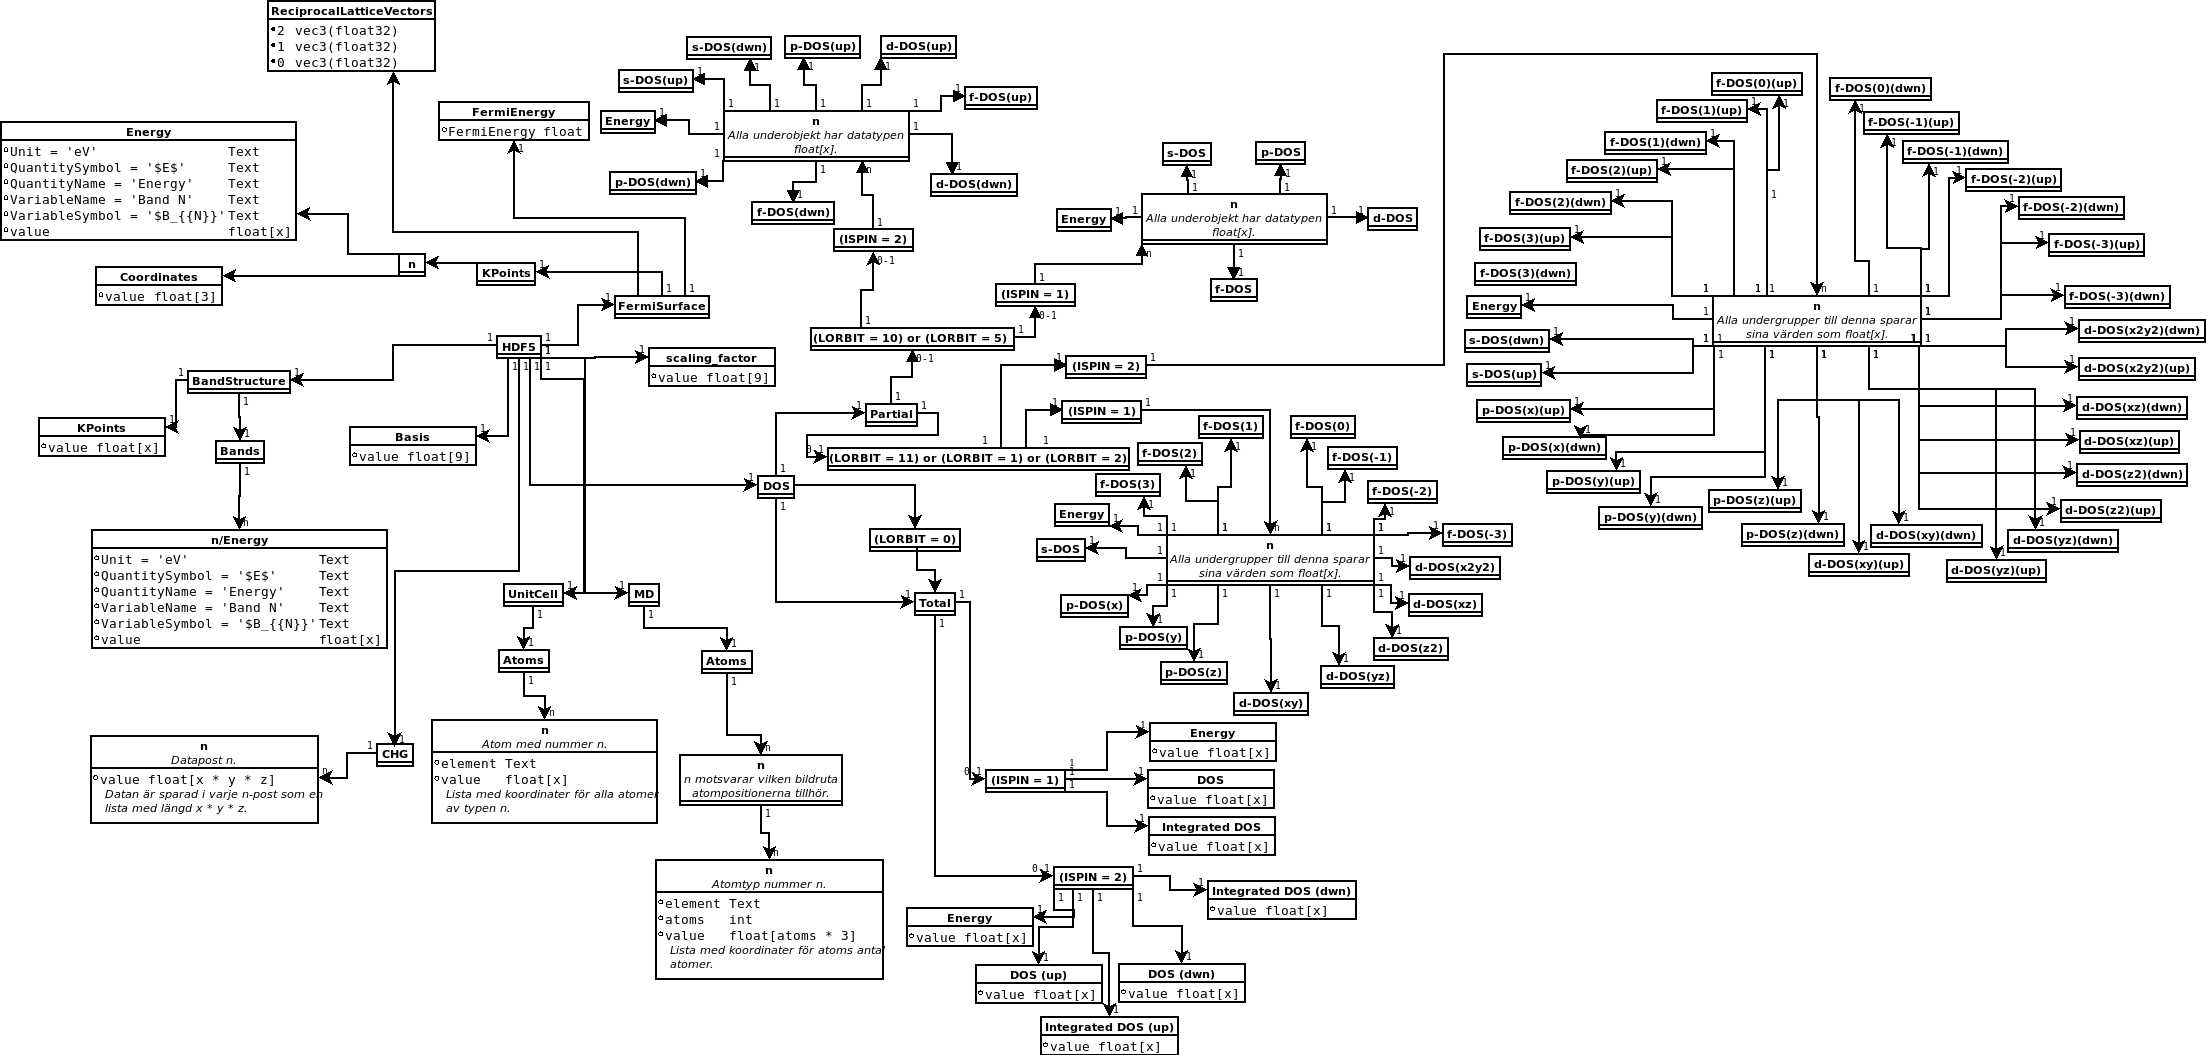
\includegraphics[scale=0.16]{hdf5-dataformat3tekdok.png}
    \caption{Dataformatet som används när VASP konverteras till HDF5.
    Se större bild i Bilaga \ref{appendix:hdf5-format} och \ref{appendix:hdf5-format2}.}
    \label{fig:hdf5-dataformat3}
\end{figure}

En ruta i diagrammet motsvarar en del i sökvägen i HDF5-objektet, om inte titeln är inom paranteser, då det innebär att rutans barnnoder blir åtkomliga om jämförelsen inom parenteserna är sann. Om en ruta har namngivna fält så innebär fältet \emph{value} den data som är sparad i ett dataset, medan övriga
datafält är attribut. En ruta som heter \emph{n}, eller har det i namnet, innebär att det finns flera dataset och att de är numrerade med heltal.

På grund av platsbrist saknar figur \ref{fig:hdf5-dataformat3} attribut för DOS-datan, men alla fält som innehåller DOS-data i diagrammet, till exempel p-DOS, d-DOS(xy), Energy, etc., har attribut som beskriver formatet på datan i fältet. En lista över attributen följer nedan:

\begin{itemize}
    \item \textbf{VariableName} är fältets namn.
    \item \textbf{VariableSymbol} är en symbol som representerar variabeln.
    \item \textbf{QuantityName} är ett för en människa läsligt namn på fältet.
    \item \textbf{QuantitySymbol} är symbol som representerar storheten.
    \item \textbf{Unit} är storhetens fysikaliska enhet.
\end{itemize}

Den högra texten i varje ruta avser alltid datatypen för en datapost. I de fall datatypen följs av hakparanteser, till exempel \emph{float[x]}, betyder det att datan är sparad i en lista där värdet inom hakparanteserna utgör listans längd.

Som exempel så koms tillståndstätheten för den totala
tillståndstätheten åt via \emph{/DOS/Total/DOS} oberoende av LORBIT. Ett till exempel är första energin för första bandet i bandstrukturen som nås via \emph{/BandStructure/Bands/0/Energy}.

\subsection{Modul för skrivning till HDF5}
Denna modul består av en pythonfil med namnet h5writer innehållandes funktionerna \_write\_coordinates, \_write\_basis, \_write\_md, \_write\_steps, \_write\_bandstruct, \_write\_dos, \_write\_volume samt \_write\_incar. Dessa funktioner skapar grupper och dataset enligt figur \ref{fig:hdf5-dataformat3} ovan. Nedan följer en kort beskrivning av varje funktion.

\textbf{\_write\_coordinates} \newline
Denna funktion skriver koordinater för atompositioner där varje atomslag tilldelas ett eget dataset. Attribut sätts för respektive grundämnesbeteckning per dataset.

Parametrar:
\begin{itemize}
\setlength\itemsep{0em}
\item h5file: Sökväg till HDF5-fil.
\item atom\_count: Lista med antalet atomer av de olika atomslagen.
\item coordinates\_list: Lista med koordinater för samtliga atomer.
\item Elements: = None eller lista med atomslag
\end{itemize}

Returnerar:
\begin{itemize}
\setlength\itemsep{0em}
\item None.
\end{itemize}

\textbf{\_write\_basis} \newline
Denna funktion skriver gittervektorerna i ett dataset med namn basis.

Parametrar:
\begin{itemize}
\setlength\itemsep{0em}
\item h5file: Sökväg till HDF5-fil.
\item basis: Lista med basvektorerna.
\end{itemize}

Returnerar:
\begin{itemize}
\setlength\itemsep{0em}
\item None.
\end{itemize}

\textbf{\_write\_bandstruct} \newline
Denna funktion skriver ut data för bandstruktur i en grupp med namn Bandstructure. Inom denna
grupp tilldelas specifika K-punkter, energier samt bandstrukturer egna dataset. Diverse attribut sätts även för bl.a. specifika energier.

Parametrar:
\begin{itemize}
\setlength\itemsep{0em}
\item h5file: Sökväg till HDF5-fil.
\item band\_data: Lista med bandstrukturdata.
\item kval\_list: Lista med K-punkter för specifika bandstrukturdata.
\end{itemize}

Returnerar:
\begin{itemize}
\setlength\itemsep{0em}
\item None.
\end{itemize}

\textbf{\_write\_dos} \newline
Denna funktion skriver ut DOS-data i en grupp med namn DOS där total och partiell DOS tilldelas grupper med namn Total respektive Partial. Inom gruppen Total tilldelas energin samt specifika DOS
egna dataset och inom gruppen Partial tilldelas varje partiell DOS egna grupper där energin samt specifika DOS tilldelas egna dataset.

Parametrar:
\begin{itemize}
\setlength\itemsep{0em}
\item h5file: Sökväg till HDF5-fil.
\item total: En lista med strängar av de olika uträkningarna som har utförts av VASP för total DOS.
\item partial: En lista med strängar av de olika uträkningarna som har utförts av VASP för partiell DOS.
\item total\_data: En lista med alla beräkningar för total DOS för varje specifik atom.
\item partial\_list: En lista med alla beräkningar för partiell DOS för varje specifik atom.
\item fermi\_energy: Fermi-energin för den aktuella uträkningen.
\end{itemize}

Returnerar:
\begin{itemize}
\setlength\itemsep{0em}
\item None.
\end{itemize}

\textbf{\_write\_volume} \newline
Denna funktion skriver ut elektrontäthetsdata och elektronlokaliseringsfunktionsdata (ELF) till grupper med namn Charge respektive Elf. Inom dessa grupper tilldelas varje iteration ett dataset.

Parametrar:
\begin{itemize}
\setlength\itemsep{0em}
\item h5file: Sökväg till HDF5-fil.
\item i: Skalär som anger numret på iterationen.
\item array: Array med parsad data för respektive iteration.
\item data\_dim: Lista som anger dimensionen av data för respektive iteration.
\item hdfgroup: En textsträng med namnet på vad man vill kalla gruppen i HDF5-filen.
\end{itemize}

Returnerar:
\begin{itemize}
\setlength\itemsep{0em}
\item None.
\end{itemize}

\textbf{\_write\_incar} \newline
Denna funktion skriver ut parsad data från INCAR i ett dataset med namn Incar där varje datatyp
tilldelas egna dataset.

Parametrar:
\begin{itemize}
\setlength\itemsep{0em}
\item h5file: Sökväg till HDF5-fil.
\item incar\_data: Datalexikon med all data från INCAR-filen.
\end{itemize}

Returnerar:
\begin{itemize}
\setlength\itemsep{0em}
\item None.
\end{itemize}

\subsection{Moduler för parsning}
Samtliga moduler för parsning består av diverse pythonfunktioner som utför själva parsningen av data. Dessa innefattar parsers som endast parsar specifika data, en som parsar INCAR-data samt en funktion som anropar samtliga parsers utom INCAR-parsern.

\subsubsection{Incarparser}
Incarparsern består av pythonfil med namnet incar som innehåller funktionerna, incar och parse\_incar. Dessa funktioner läser in och sparar information från INCAR-filen samt anropar en separat pythonmodul som skriver en HDF5-fil. INCAR är en inputfil för VASP som anger hur VASP ska exekvera elektronberäkningar. VASP-användaren har initialt satt värden rad för rad för en mängd variabler.

Funktionen incar kontrollerar om HDF5-filen redan innehåller INCAR-data och anropar funktionen parse\_incar om så inte är fallet. Existerar INCAR-filen i användarens VASP-katalog parsas data av funktionen parse\_incar som då sparar ett dataset för varje datatyp och namnger dataseten därefter. Funktionen incar anropar sedan pythonmodulen som skriver HDF5-filen där varje enskilt dataset tilldelas en egen grupp (se delavsnitt \ref{ch:hdf5struktur} ovan för beskrivning av strukturen i HDF5-filen).

Funktionsanrop: envision.parser.vasp.incar(h5file, vasp\_dir)

Parametrar:
\begin{itemize}
\setlength\itemsep{0em}
\item h5file: Sökväg till HDF5-fil.
\item vasp\_dir: Sökväg till VASP-katalog.
\end{itemize}

Returnerar:
\begin{itemize}
\setlength\itemsep{0em}
\item Lista med namn på data (dataseten) som parsats.
\item Bool: True om parsning skett felfritt, False annars.
\end{itemize}

\subsubsection{Volymparser}
Volymparsern består av en mängd funktioner i en pythonfil som används för parsning av CHG och ELFCAR. Den kan läsa in och spara data på HDF5-format från båda dessa filer genom att anropa en pythonmodul. Detta är för att CHG och ELFCAR har samma struktur och består av ett antal iterationer av volymdata från volymberäkningar. Således innehåller den sista iterationen data som är mest korrekt. Därför skapar volymparsern också en länk till den sista iterationen i HDF5-filen för att data av högst kvalitet lätt ska kunna plockas ut.

Funktionsanrop vid parsning av CHG-data: envision.parser.vasp.charge(h5file, vasp\_dir)

Funktionsanrop vid parsning av ELFCAR-data: envision.parser.vasp.elf(h5file, vasp\_dir)

Parametrar:
\begin{itemize}
\setlength\itemsep{0em}
\item h5file: Sökväg till HDF5-fil.
\item vasp\_dir: Sökväg till VASP-katalog.
\end{itemize}

Returnerar:
\begin{itemize}
\setlength\itemsep{0em}
\item Bool: True om parsning skett felfritt, False annars.
\end{itemize}

\subsubsection{Tillståndstäthetsparser}
\label{ch:dosparser}
Tillståndstäthetsparsern består av en mängd funktioner i en pythonfil som används för parsning av DOSCAR. DOSCAR-filen består först av den totala tillståndstätheten och sedan partiell tillståndstäthet för varje atom i kristallen. Beroende på vad som står i INCAR kan dock denna data se väldigt olika ut. Flaggorna ISPIN, RWIGS och LORBIT i INCAR-filen avgör vad som skrivs i DOSCAR-filen. ISPIN-flaggan informerar om spinn har tagits hänsyn till vid beräkningar, RWIGS-flaggan specificerar Wigner-Seitz-radien för varje atomtyp och LORBIT-flaggan (kombinerat med RWIGS) avgör om PROCAR- eller PROOUT-filer (som DOSCAR-filen refererar till) skrivs. Parsern läser därför från data givet av incarparsern i HDF5-filen för att se hur DOSCAR ska parsas.
Parsern delar upp data i två grupper i HDF5-filen, total och partiell. I gruppen partiell finns det en grupp för varje atom. Ett dataset för varje undersökt fenomen skrivs sedan ut för varje atom under partiell, och för total tillståndstäthet under total.

Funktionsanrop: envision.parser.vasp.dos(h5file, vasp\_dir)

Parametrar:
\begin{itemize}
\setlength\itemsep{0em}
\item h5file: Sökväg till HDF5-fil.
\item vasp\_dir: Sökväg till VASP-katalog.
\end{itemize}

Returnerar:
\begin{itemize}
\setlength\itemsep{0em}
\item Bool: True om parsning skett felfritt, False annars.
\end{itemize}

% TODO: Lägg tll detta om vi behandlar Fermi.
\iffalse
\subsubsection{Fermi-yteparser}
Fermi-yteparsern består av en mängd funktioner i en pythonfil som används för parsning av OUTCAR och EIGENVAL. OUTCAR-filen parsas för att hitta Fermi-energin och basvektorer för den irreducibla 1:a Brillouin-zonen i kartesiska koordinater. EIGENVAL-filen parsas för varje k-punkts energivärden för varje band.

Funktionsanrop: envision.parser.vasp.fermi(h5file, vasp\_dir)
\fi

Parametrar:
\begin{itemize}
\setlength\itemsep{0em}
\item h5file: Sökväg till HDF5-fil.
\item vasp\_dir: Sökväg till VASP-katalog.
\end{itemize}

Returnerar:
\begin{itemize}
\setlength\itemsep{0em}
\item Bool: True om parsning skett felfritt, False annars.
\end{itemize}

\subsubsection{Enhetscellsparser}
Enhetscellparsern läser in gittervektorer, som multipliceras med skalfaktorn och skrivs till /basis i HDF5-filen. Atompositioner läses från POSCAR och om dessa är angivna med kartesiska koordinater räknas de om till koordinater med gittervektorerna som bas. Koordinaterna skrivs till HDF5-filen uppdelade efter atomslag och attribut sätts med respektive grundämnesbeteckning. Om dessa inte ges med parametern elements letar parsern i första hand i
POTCAR och i andra hand i POSCAR.

Funktionsanrop: envision.parser.vasp.unitcell(h5file, vasp\_dir, elements = None)

Parametrar:
\begin{itemize}
\setlength\itemsep{0em}
\item h5file: Sökväg till HDF5-fil.
\item vasp\_dir: Sökväg till VASP-katalog.
\item elements = None: None eller lista med atomslag.
\end{itemize}

Returnerar:
\begin{itemize}
\setlength\itemsep{0em}
\item Bool: True om parsning skett felfritt, False annars.
\end{itemize}

\subsubsection{parse\_all}
parse\_all är en funktion för parsning av allt som finns i katalogen som ges som inparameter. Funktionen kallar på alla systemets parsers och skriver ut meddelande om vad som parsas och om
parsningen gjordes eller ej. Den returnerar en lista med alla namn på grupper i HDF5-filen eller None om HDF5-filen ej skapats.

Funktionsanrop: envision.parse\_all(h5\_path, dir)

Parametrar:
\begin{itemize}
\setlength\itemsep{0em}
\item h5\_path: Sökväg till HDF5-fil.
\item vasp\_dir: Sökväg till katalog med utdata-filer från beräkningsprogram.
\end{itemize}

Returnerar:
\begin{itemize}
\setlength\itemsep{0em}
\item Bool: True om parsning skett felfritt, False annars.
\end{itemize}

\section{Delsystem 2 - System för visualisering}
Visualiseringssystemet består av ett antal pythonmoduler för nätverksbygge i Inviwo samt c++-moduler implementerade i Inviwo av projektgruppen för att visualisera data.

\subsection{Nätverk}
Processorer är de primära objekt i nätverken som användaren interagerar med. De består bland annat av inportar och utportar som används vid utbyte av data av specifika typer. Nätverken mynnar ut i en så 
kallad Canvas, en processor som på sin inport tar rastergrafikdata som den visualiserar i ett separat fönster. Samtliga pythonmoduler som bygger nätverk består i huvudsak av kod som anropar Inviwos egna interna funktioner för att bland annat importera, koppla, länka samt sätta värden på specifika parametrar i processorer.

\subsubsection{Nätverk för visualisering av volymdata}
\label{ref:visualisering-volymdata}

Data som visualiseras med hjälp av volymnätverket är elektrontäthetsdata och 
elektronlokaliseringsfunktionsdata (ELF-data).
Nätverket kan visualisera 
data med hjälp av tekniken volume ray casting eller iso ray casting. 
Se figur \ref{fig:screenshot_elf} nedan som visar en skärmbild
från Inviwo när visualisering av ELF-data
för diamant
med iso ray casting görs. Det tillhörande nätverket syns i figur \ref{fig:screenshot_elf_network}.

\begin{figure} [H]
\centering
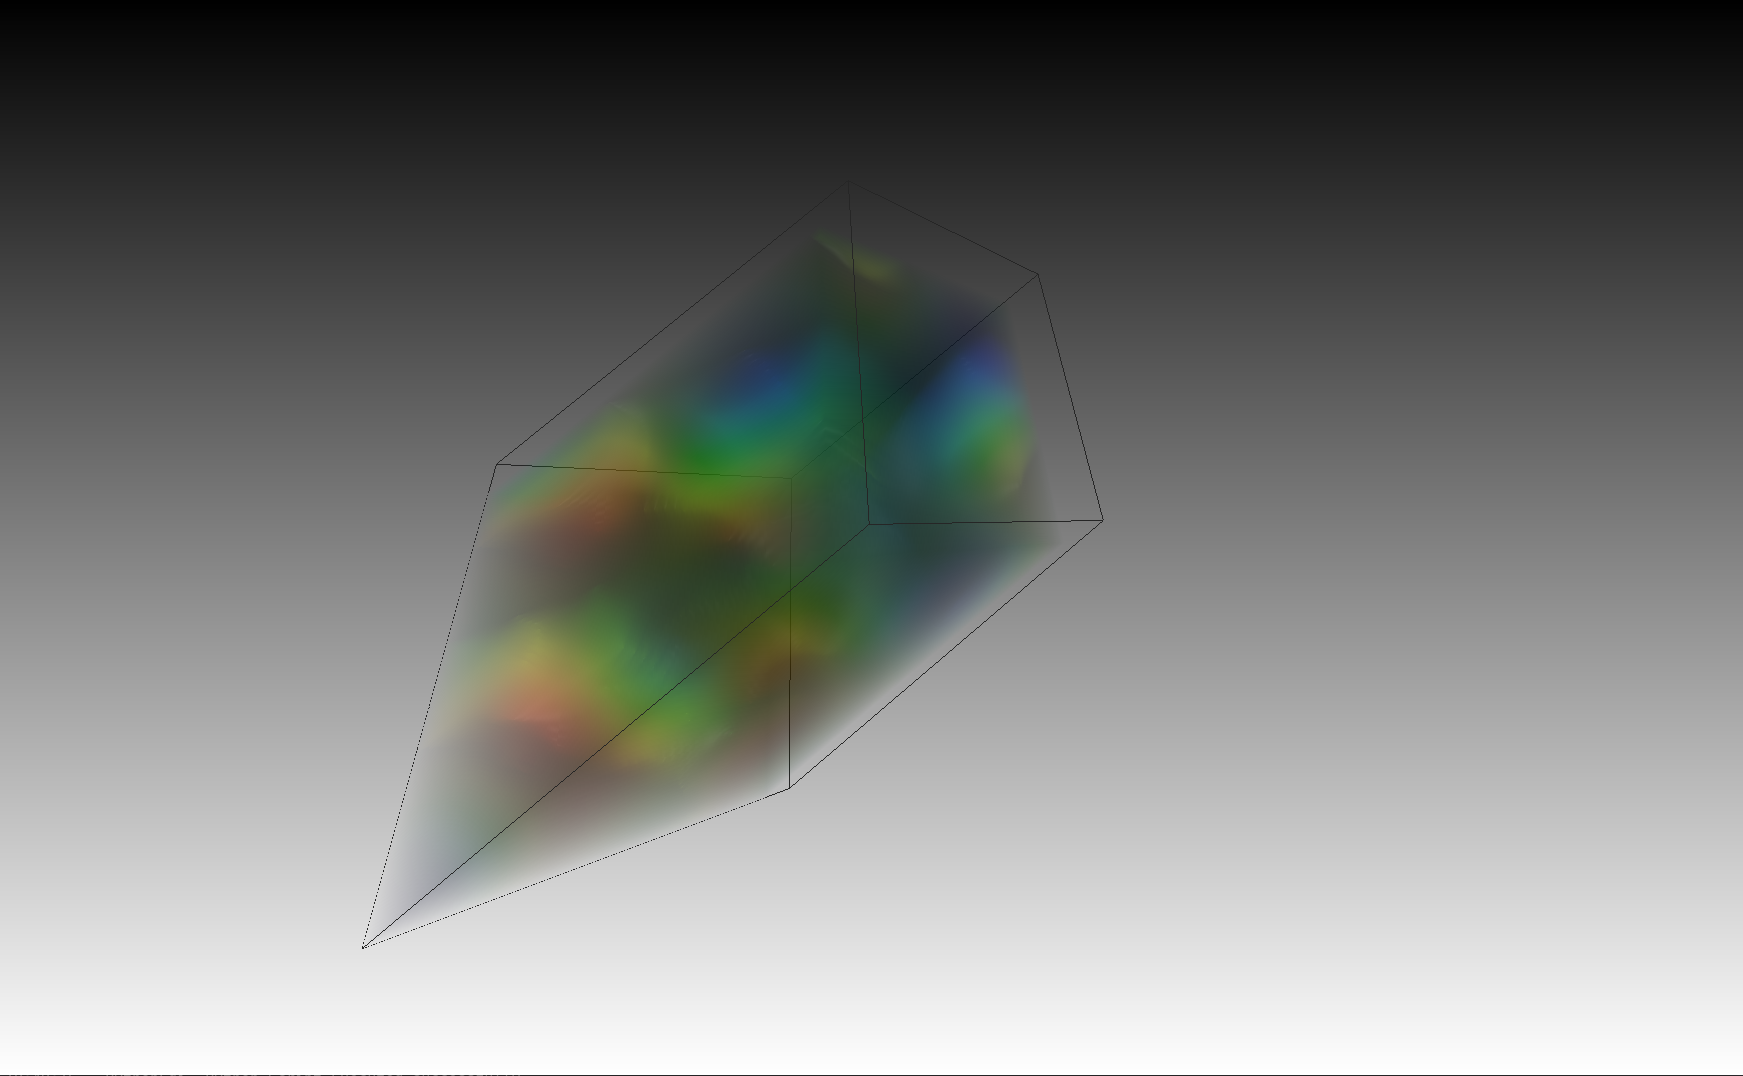
\includegraphics[scale = 0.25]{screenshot_elf_diamant.png}
\caption{Visualisering av ELF-data för diamant i Inviwo.}
\label{fig:screenshot_elf}
\end{figure}

\begin{figure} [H]
\centering
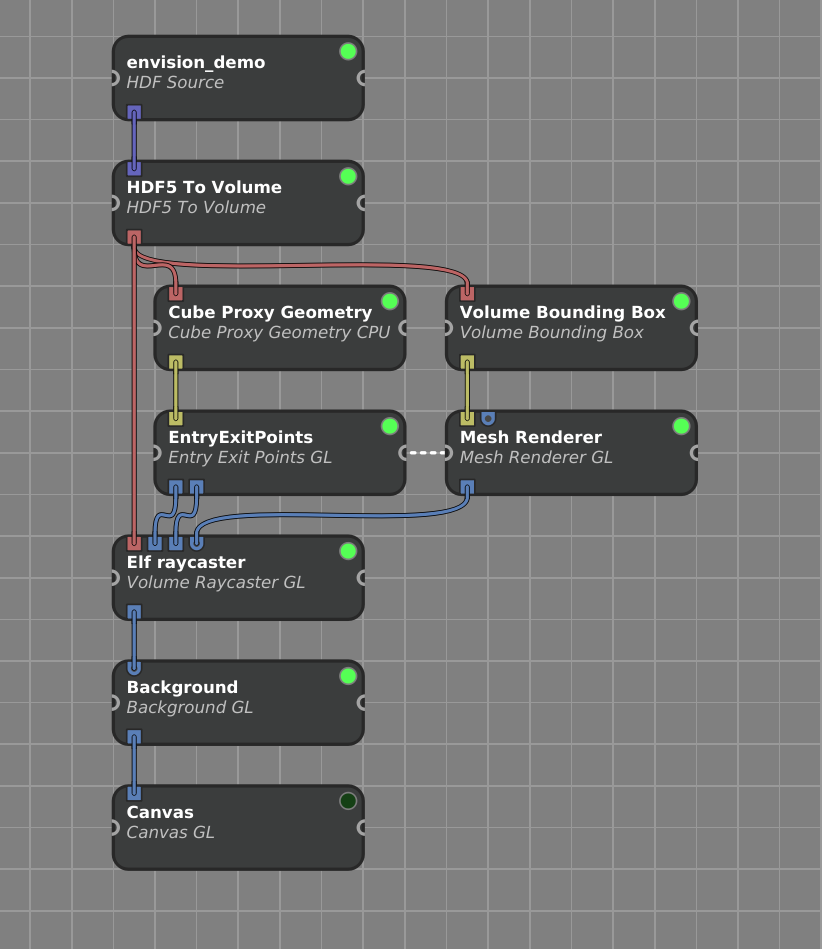
\includegraphics[scale=0.4]{screenshot_elfnatverk_diamant.png}
\caption{Nätverket för visualisering av ELF-data för diamant i Inviwo}
\label{fig:screenshot_elf_network}
\end{figure}

När tekniken volume ray casting
används har användaren möjlighet att 
aktivera en slice-funktion som skapar
ett plan som skär
igenom volymen. 
Visualiseringen består då av två stycken bilder placerade 
bredvid varandra i samma Canvas.
Högra bilden visar hela volymen tillsammans med ett plan, som användaren på eget behag kan flytta, och 
vänstra bilden visar utseendet av det specifika tvärsnitt av volymen som planet i varje enskild position 
skapar. 
Se figur \ref{fig:screenshot_NaCl_laddningstathetslice} nedan som visar en skärmbild från Inviwo 
när visualisering av laddningstäthet för natriumklorid, NaCl,
med volume ray casting
och slice-funktion görs, och figur \ref{fig:screenshot_NaCl_laddningstathetslicenatverk} för tillhörande nätverk. Försöker användaren visualisera data 
med iso ray casting och slice-funktion returneras meddelandet ``Slice is not possible with ISO 
Raycasting, therefore no slice-function is showing.” och en visualisering med iso ray casting utan slice-funktion görs. Figur \ref{fig:screenshot_NaCl_laddningstathet_iso} visar visualisering av laddningstäthet för NaCl med ISO ray casting, där en isoyta ritats upp för laddningstäthet lika med 0.15.

\begin{figure} [H]
\centering
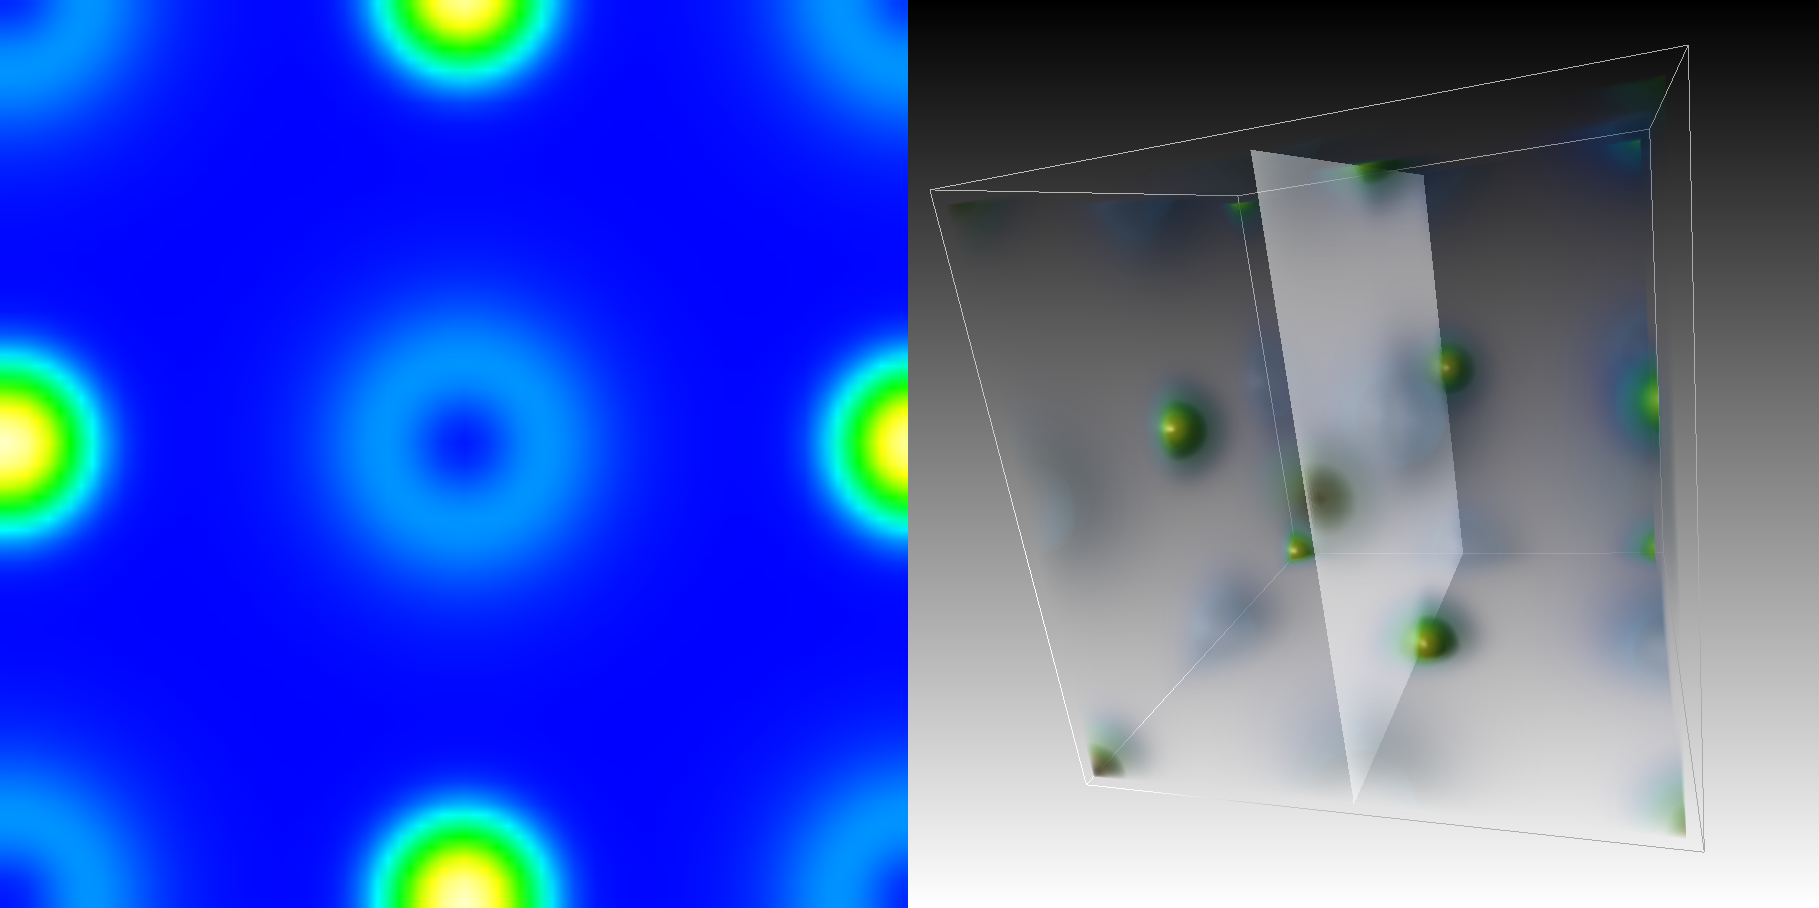
\includegraphics[scale=0.25]{screenshot_NaCl_laddningstathetslice.png}
\caption{Visualisering av laddningstäthet för NaCl med slice-funktion i Inviwo.}
\label{fig:screenshot_NaCl_laddningstathetslice}
\end{figure}

\begin{figure} [H]
\centering
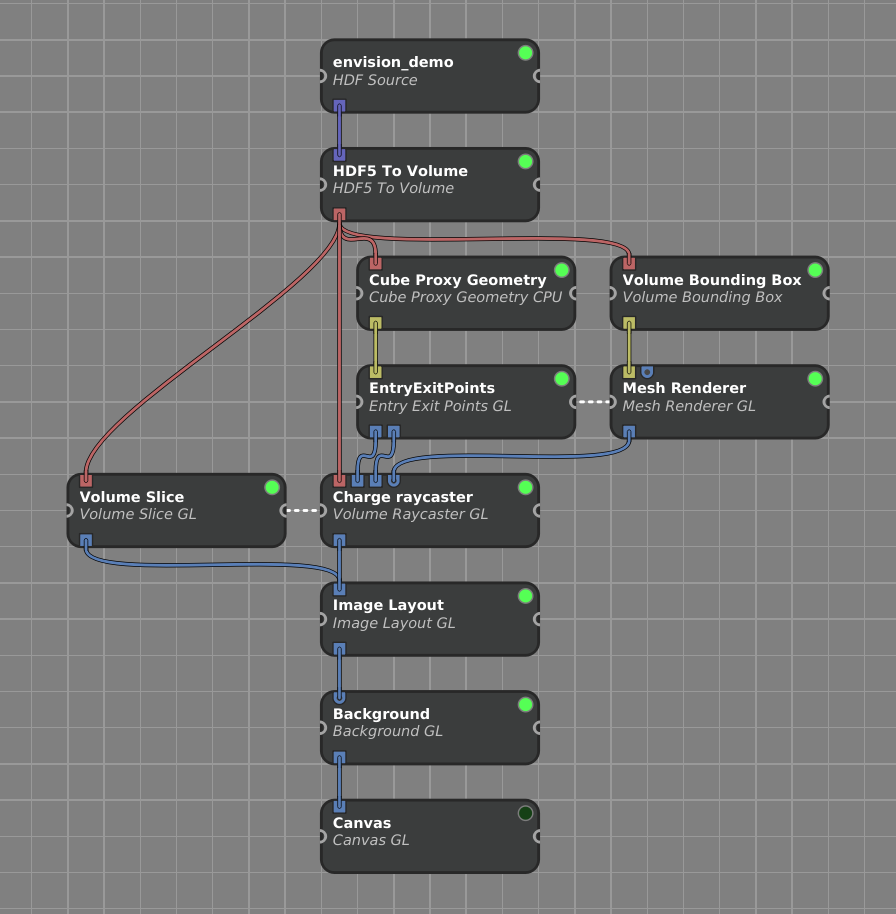
\includegraphics[scale=0.4]{screenshot_NaCl_laddningstathetslicenatverk.png}
\caption{Nätverket för visualisering av laddningstäthet för NaCl med slice-funktion i Inviwo.}
\label{fig:screenshot_NaCl_laddningstathetslicenatverk}
\end{figure}

\begin{figure} [H]
\centering
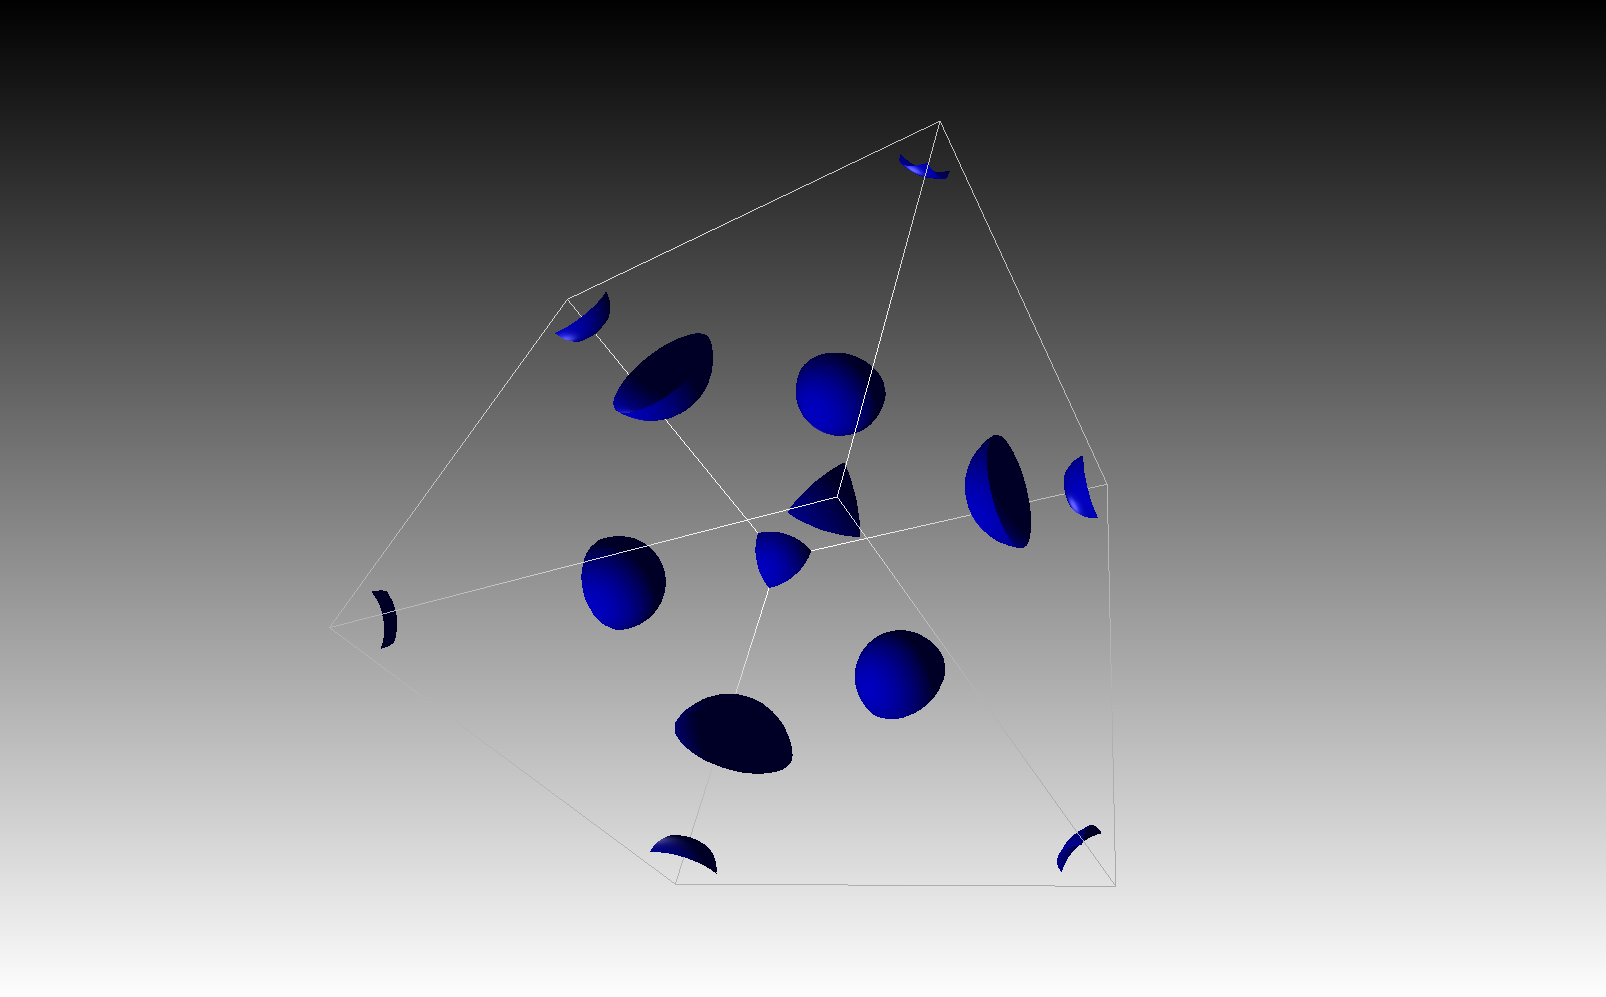
\includegraphics[scale=0.3]{screenshot_NaCl_laddningstathet_iso.png}
\caption{Visualisering av laddningstäthet för NaCl med ISO raycasting.}
\label{fig:screenshot_NaCl_laddningstathet_iso}
\end{figure}

Systemet som bygger volymnätverket består av en pythonfil med namnet volume
innehållandes tre funktioner: charge, elf och volume\_network.

Funktionerna charge och elf är de funktioner som användaren anropar och de tar vardera fem argument:

\begin{itemize}
\item h5file: Sökvägen till HDF5-filen där samtlig data finns.
\item iso: Önskas iso-yta
sätts denna till det specifika värdet iso-ytan ska ha annars till None. Defaultvärde = None.
\item slice: Bool-variabel som sätts till True om slicefunktion önskas, annars till False.
\item xpos: Den översta processorns x-koordinat. Default = 0.
\item ypos: Den översta processorns y-koordinat. Default = 0.
\end{itemize}

Funktionsanrop charge: \newline
envision.inviwo.charge(h5file, iso = None,
slice = False, xpos = 0, ypos = 0)

Funktionsanrop ELF: \newline
envision.inviwo.elf(h5file, iso = None
, slice = False, xpos = 0, ypos = 0) \newline

Dessa två funktioner anropar funktionerna volume\_network som bygger själva nätverket. Denna tar argumenteten:

\begin{itemize}
\item h5file: Sökvägen till HDF5-filen där samtlig data finns.
\item volume: En textsträng som anger om elektrontäthetsdata eller ELF-data ska visualiseras.
\item iso: Önskas iso-yta sätts denna till det specifika värde iso-ytan ska ha annars till None.
\item slice: Bool-variabel som sätts till True om slicefunktionen önskas, annars False.
\item xstart\_pos: Den översta processorns x-koordinat.
\item ytart\_pos: Den översta processorns y-koordinat.
\end{itemize}

Funktionen charge anropar användaren för att visualisera elektrontäthet och funktionen elf för att visualisera ELF-data. Båda dessa anger argumentet ``h5file” i funktionen volume\_network 
med det värde användaren gett som argument 
``h5file” till respektive funktion som. Argumentet ``volume” anger funktionen charge som ``Charge raycaster” och funktionen elf som ``Elf raycaster”. 
Resterande argument sätts, på samma sätt som för argumentet ``h5file”, till det värde användaren gett motsvarande argument till respektive funktion.

Funktionen volume\_network laddar en HDF Source processor som ges samma namn som HDF5-filen. 
Dess utdata skickas till en HDF5 To Volume processor. HDF Source processorn anger vilken HDF5-fil och HDF5 To Volume processorn anger, baserat på argumentet ``volume”,
vilken specifik grupp i HDF5-filen som data ska laddas från. Utdata från HDF5 To Volume processorn skickas till processorerna Cube Proxy Geometry, Volume Bounding Box samt till processorn för ray casting. Baserat på 
argumentet ``iso” laddas processorn ISO Raycaster eller Volume Raycaster och denna ges namnet 
``Charge raycaster” eller ``Elf raycaster” baserat på argumentet ``volume”. Processorn Cube Proxy 
Geometry skapar en proxy geometri i form av en mesh formad som en parallellepiped
och skickar denna data till processorn Entry Exit Points. Denna processor beräknar start- och slutpunkt för respektive ”stråle där data samplas från” i processorn för ray casting och utgör således en del av denna processors indata. Beräkningen av start- och slutpunkt görs utgående från aktuell vinkel som den 
kamera som ``ser in i” volymen data representerar har. Processorn Volume Bounding Box definierar 
geometrin för en mesh som omsluter volymen (utgör dess kanter) och skickar denna data till 
processorn Mesh Renderer som skapar meshen. Mesh Renderer skickar sedan denna data till 
processorn för ray casting.

Baserat på utdata från processorerna HDF5 To Volume, Entry Exit Points och Mesh Renderer skapar 
sedan processorn för ray casting en 2-dimensionell representation av volymen som data representerar. 
Denna data skickas, via processorn Background som lägger till en bakgrund, till Canvas-processorn. Se figur \ref{fig:screenshot_elf_network} som visar en skärmbild från Inviwo över nätverket när ELF-data för diamant visualiseras med volume ray casting.

Om slicefunktionen används laddar även funktionen volume\_network en Volume Slice processor och en Image Layout processor. Volume Slice processorn skapar det plan som skär volymen se figur \ref{fig:screenshot_NaCl_laddningstathetslice} till höger.
Indata till denna processor utgörs av utdata från HDF5 To Volume processorn och dess utdata 
går till processorn Image Layout. Processorn Image Layout skapar en delad vy över de båda bilderna 
se figur \ref{fig:screenshot_NaCl_laddningstathetslice}
ovan och dess indata utgörs, förutom av utdata från Volume Slice processorn, av utdata 
från processorn för ray casting. Denna data skickas sedan, via processorn Background som skapar en 
bakgrund, till Canvas-processorn. Se figur \ref{fig:screenshot_NaCl_laddningstathetslicenatverk} som visar en skärmbild från Inviwo över nätverket när laddningstäthet för natriumklorid, NaCl, visualiseras med hjälp av volume ray casting och slice-funktion.

\subsubsection{Nätverk för visualisering av enhetscell} 
Funktionen för visualisering av enhetscell
placerar ut en koordinatläsarprocessor (CoordinateReader) per atomslag och kopplar dessa till en processor av typen HDF source, som läser den av användaren angivna HDF5-filen. Utdata från koordinatläsarna skickas till en StructureMesh-processor som placerar ut klot som representerar atomer. Färg och radie sätts enligt en fördefinierad lista, men kan ändras via Inviwos grafiska användargränssnitt. Utdata från 
StructureMesh skickas till processorn Sphere Renderer,
som sköter själva renderingen. 
Utporten på denna processor kan kopplas till den blå inporten på processorn Mesh Renderer i 
volymrenderingsnätverket, se delavsnittet \ref{ref:visualisering-volymdata} om detta nätverk ovan, 
så att enhetscellen visas tillsammans 
med elektronstrukturen. Se figur \ref{fig:enhetscell}
nedan som vardera visar en skärmbild från Inviwo när 
visualisering av enhetscell 
för titanfosfat (TiPO4) görs, och figur \ref{fig:enhetscellnatverk} för tillhörande nätverk.

\begin{figure}[H]
    \centering
    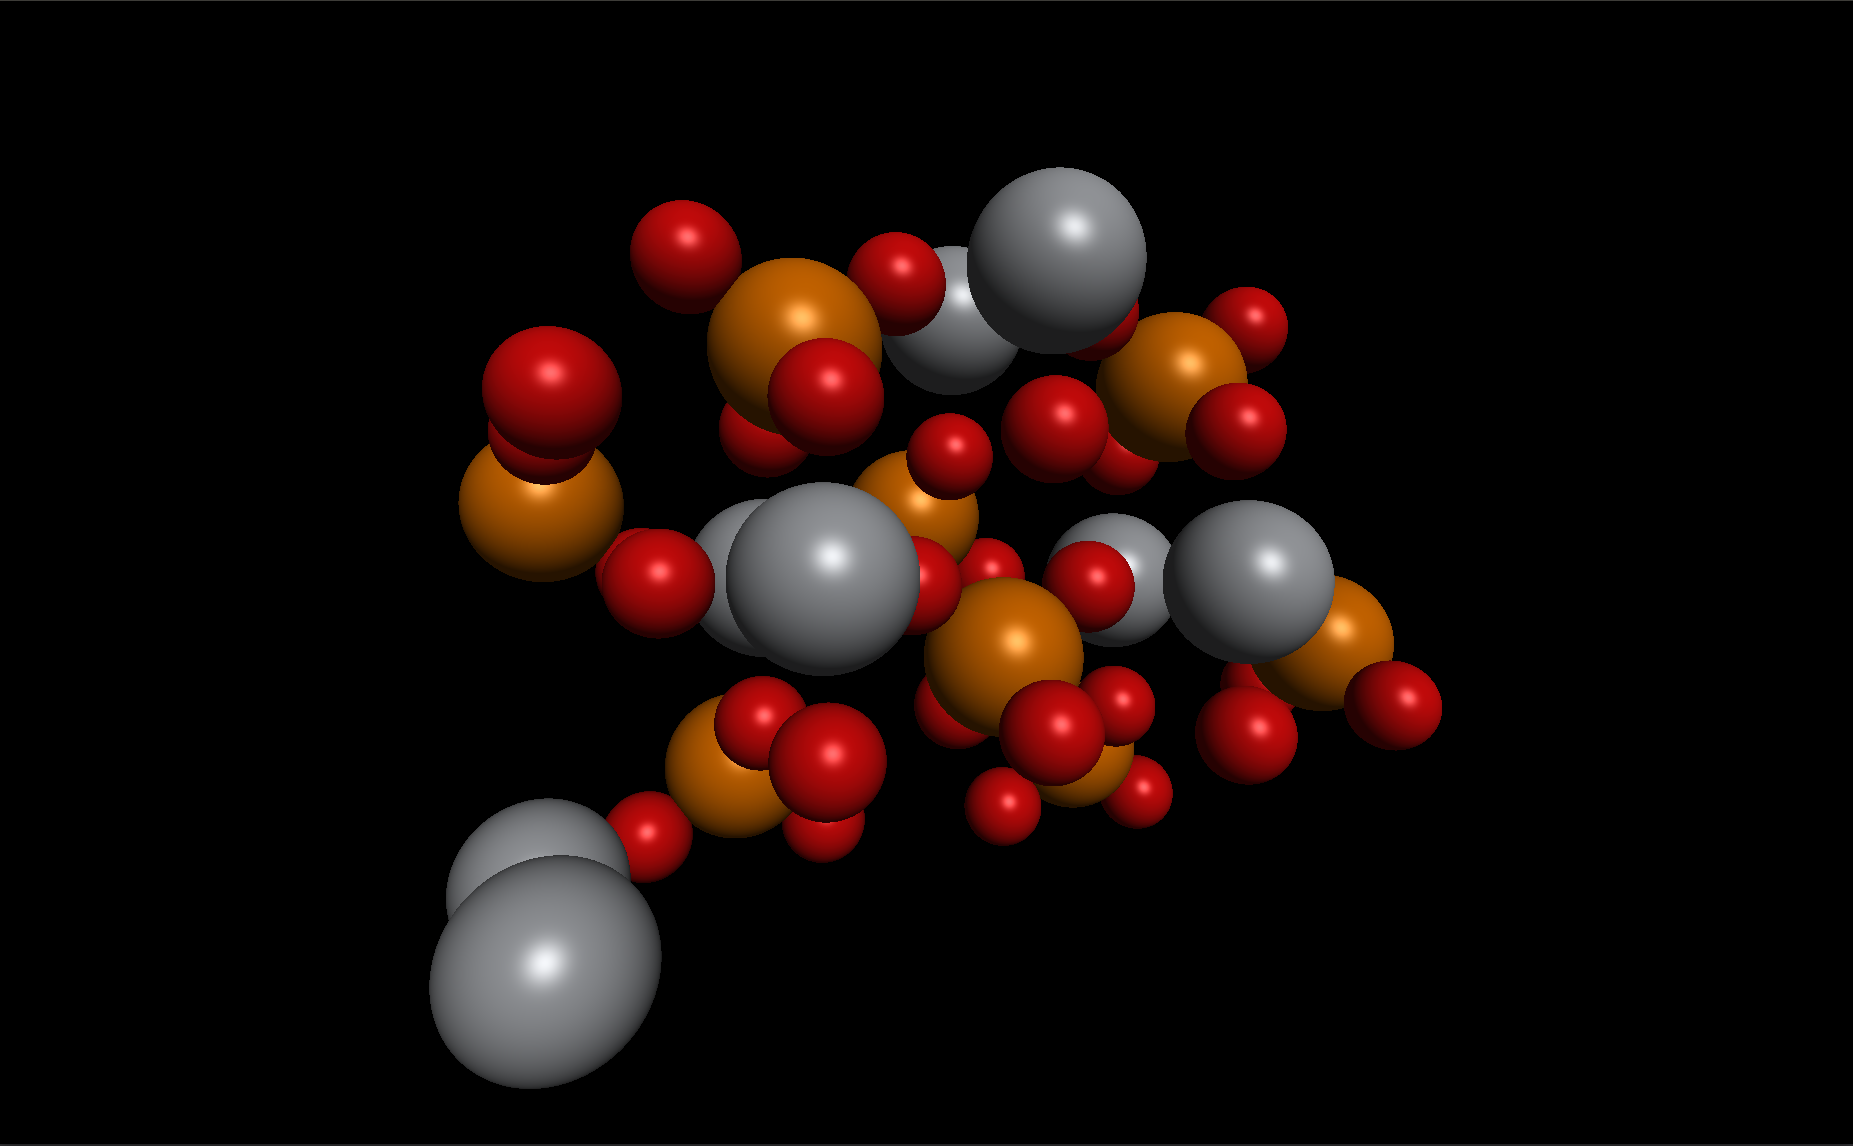
\includegraphics[scale=0.25]{screenshot_enhetscell_TiPO4.png}
    \caption{Visualisering av TiPO4 i Inviwo}
    \label{fig:enhetscell}
\end{figure}

\begin{figure}[H]
    \centering
    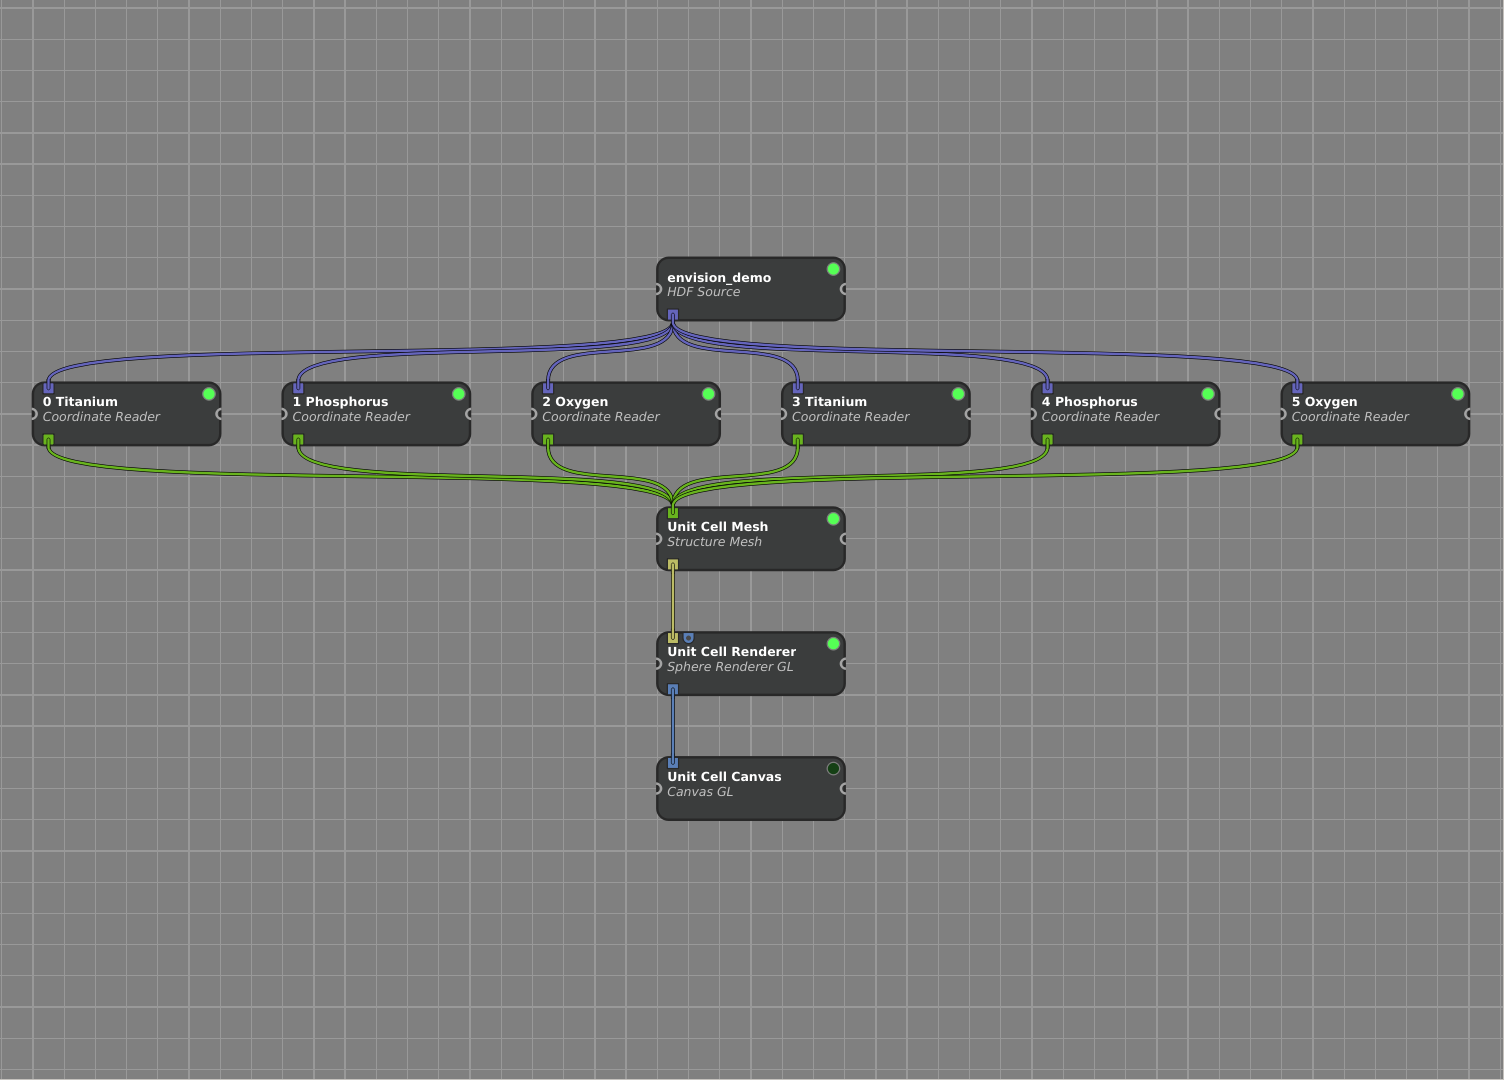
\includegraphics[scale=0.30]{screenshot_enhetscellnatverk_TiPO4.png}
    \caption{Nätverket för visualisering av TiPO4 i Inviwo.}
    \label{fig:enhetscellnatverk}
\end{figure}

\subsubsection{Nätverk för visualisering av DOS}
Nätverket för visualisering av tillståndstäthetsdata laddar en HDF Source processor som anger HDF5-filen som data laddas från om HDF Source processor inte finns, annars kopplas
en HDF5 Path Selection processor, som tar ut den givna HDF5-gruppens alla undergrupper (beskrivs närmare i kap. \ref{ch:processorer}) direkt till den redan befintliga HDF Source processorn. Denna processor anger att data ska laddas från DOS-gruppen i HDF5-filen. Två till HDF5 Path Selection processorer laddas sedan som anger grupperna Total och Partial i HDF5-filen.  

För Total-delen laddas sedan kontinuerligt HDF5 To Function processorer som gör funktioner av all 
data i Total-gruppen. För Partial-gruppen laddas en HDF5 Path Selection processor (beskrivs närmare i kap. \ref{ch:hdf5-processorer}) som tar ut dataset för en vald atom genom att välja den givna HDF5-filens relevanta undergrupp. Denna processor har namnet Partial Pick i nätverket. Därefter laddas HDF5 To Function
processorer för alla dataset i 
grupperna under Partial-gruppen. All data matas sedan i en
lineplot processor (beskrivs närmare i kap. \ref{ch:2d-processorer}) som gör en 2D-graf. Detta matas in i en Canvas-processor som visar själva grafen. Dessutom finns två textOverlay processorer som skriver ut text för x- och y-axeln. Figur \ref{fig:total_dos} visar total tillståndstäthet för koppar, Cu. Skärmbilden i figur \ref{fig:network_dos} är över nätverket som ger 2D-grafen i figur \ref{fig:total_dos}, nätverket ger även en 2D-graf av den partiella tillståndstätheten.

\begin{figure}[H]
    \centering
    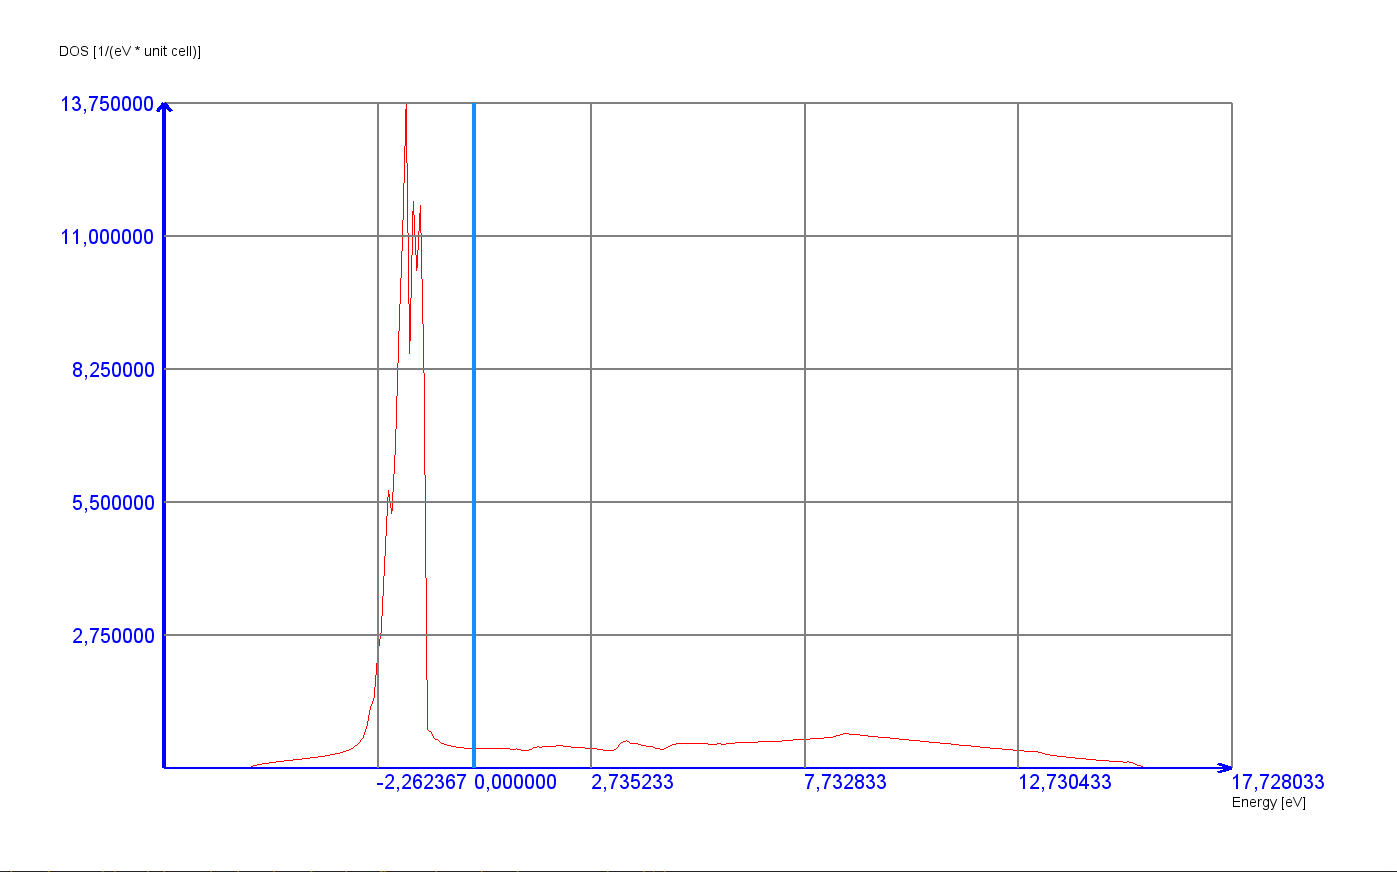
\includegraphics[scale=0.30]{screenshot_total_dos_Cu_1_10.png}
    \caption{Visualisering av Total DOS för Cu.}
    \label{fig:total_dos}
\end{figure}

\begin{figure}[H]
    \centering
    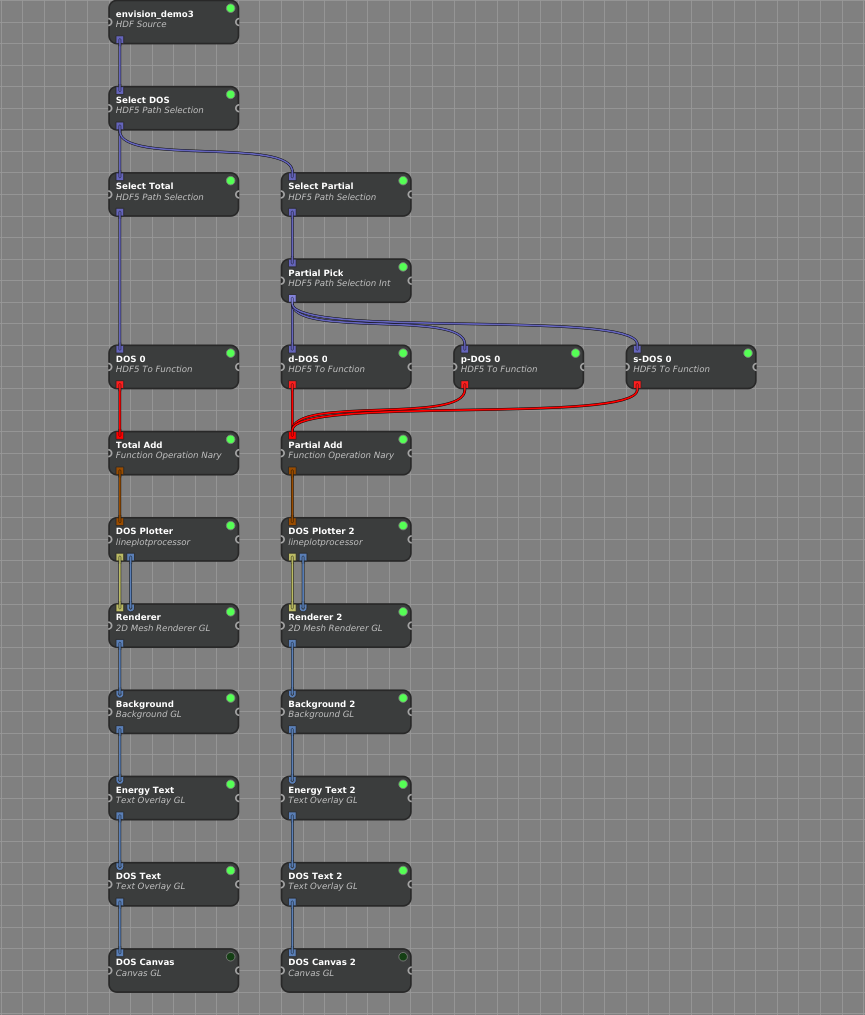
\includegraphics[scale=0.35]{screenshot_dos_network_Cu_1_10.png}
    \caption{Nätverket för visualisering av total och partiell tillståndstäthet för Cu.}
    \label{fig:network_dos}
\end{figure}

Det går att visualisera dos tillsammans med visualisering av kristallstruktur och med hjälp av en så kallad ''picking''-funktion välja enskilda atomer för att se tillhörande tillståndstäthet. Mer om detta i kap. \ref{ch:sammankoppling}.

\subsubsection{Sammankoppling av nätverk}
\label{ch:sammankoppling}
Alla de typer av visualisering som är listade ovan kan köras samtidigt, oberoende av varandra, så länge nödvändig data återfinns i de tillhandahållna VASP-filerna. Funktionalitet för att koppla ihop nätverk med varandra och visualisera flera egenskaper i samma bild finns för några kombinationer av egenskaper. Alla kombinationer av tredimensionell visualisering i det ``direkta'' rummet (alltså inte det reciproka rummet) kan fås i samma bild. Ett exempel på detta är figur \ref{fig:sammankoppling} som visar visualisering av enhetscellsdata och ELF-data för aluminium, Al, i samma bild.

\begin{figure} [H]
\centering
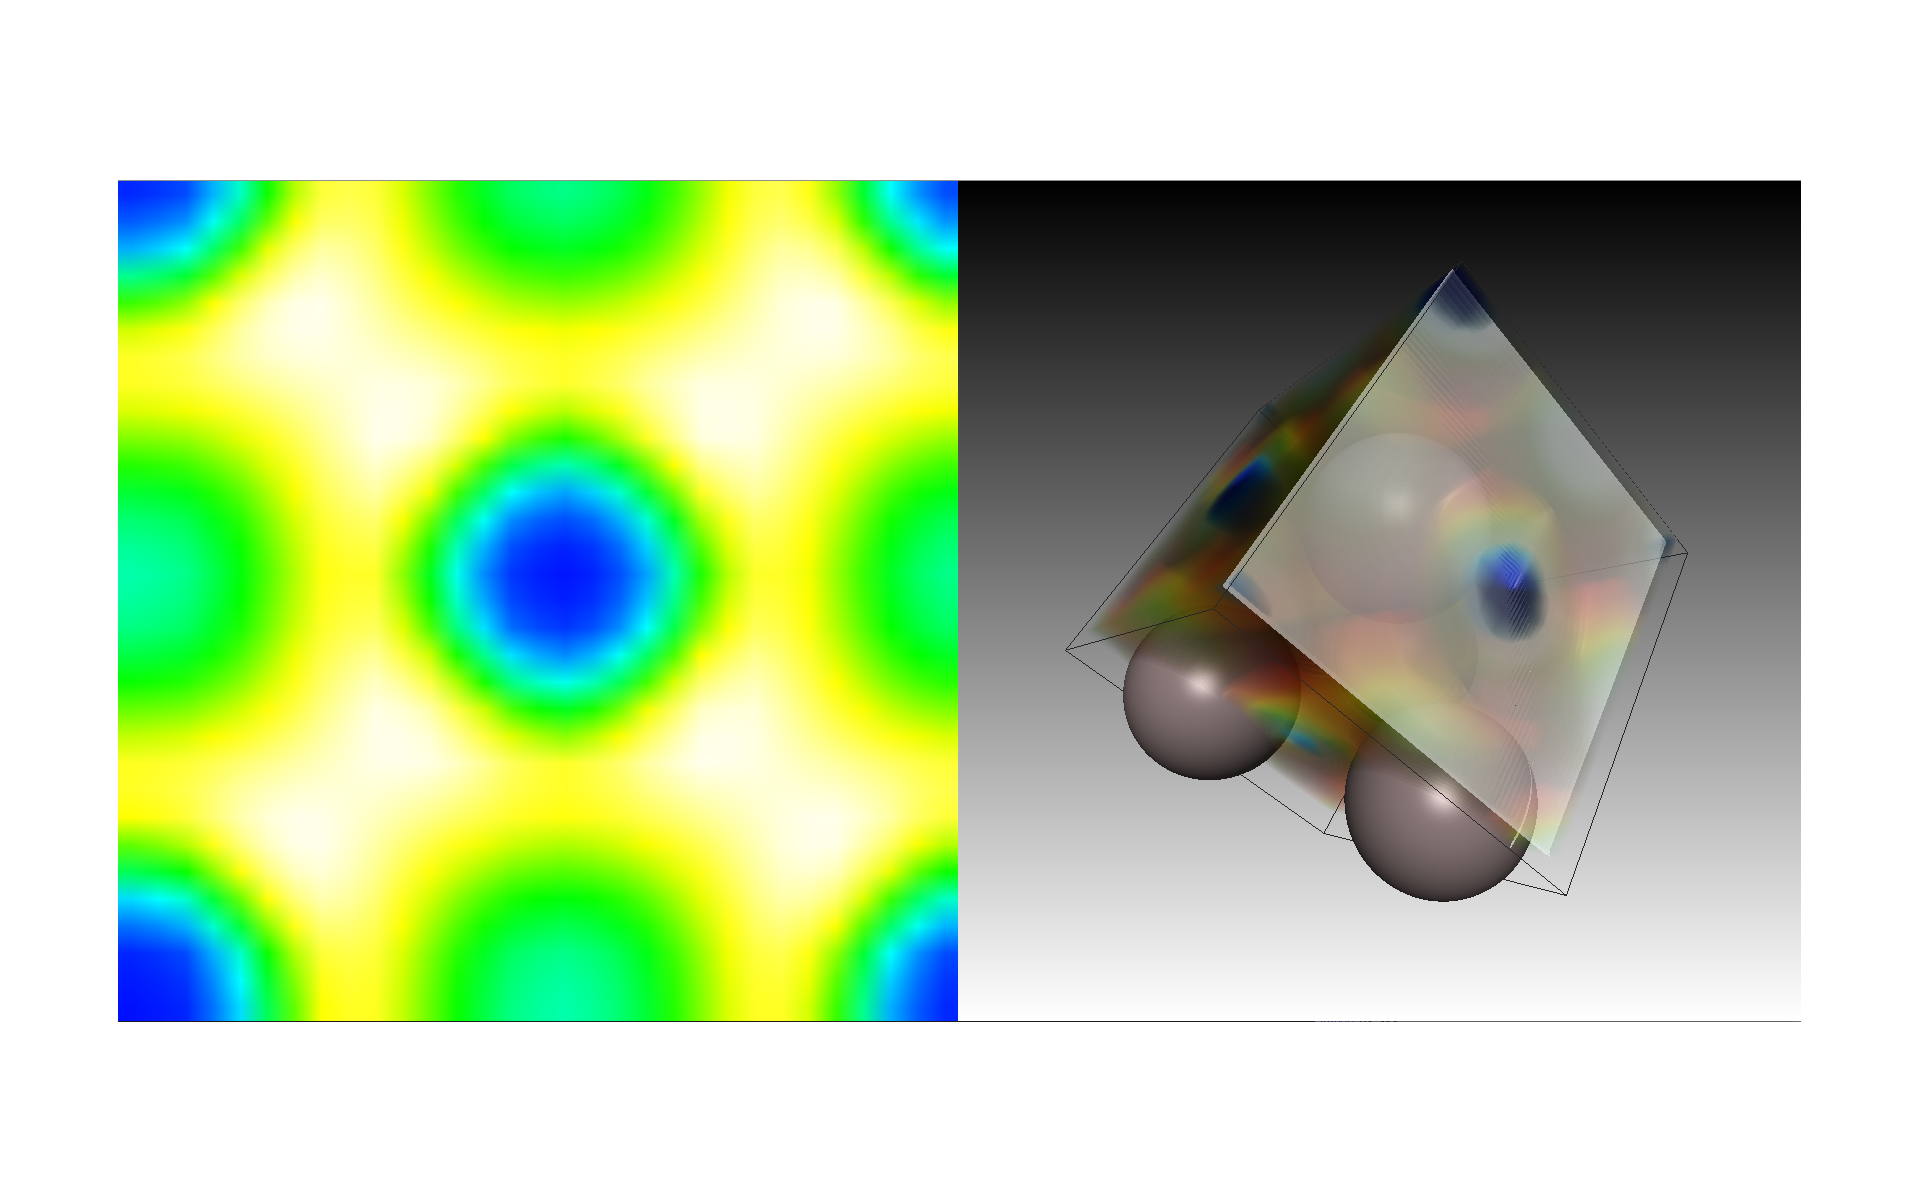
\includegraphics[scale=0.25]{screenshot_sammankoppling_Al.png}
\caption{Data för enhetscell och ELF för aluminium visualiserat i samma bild, med volume ray casting och slice-funktion. Slice-funktionens plan är här placerat alldeles intill enhetscellens sida.}
\label{fig:sammankoppling}
\end{figure}

\textbf{\textit{DOS sammankopplat med enhetscell}}\newline
DOS och enhetscellen kan visualiseras samtidigt och ger då en bild med kristallstrukturen till vänster och tillståndstätheten åt höger. Då möjliggör en ''picking''-funktion att användaren kan trycka på enskilda atomer för att få ut den projicerade tillståndstätheten. Processorn StructureMesh har en BoolProperty med namnet enablePicking\_ (se kap. \ref{ch:kristallstruktur-processorer}), sätts denna till True så blir det möjligt att välja enskilda atomer i enhetscellen genom att klicka på dem. 

Om en processor med namnet ''Unit Cell Mesh'' hittas i nätverket så byts Partial Pick All mot Partial Pick och i Unit Cell Mesh sätts enblePicking\_ till True efter att Partial Picks:s property intVectorProperty\_ och Unit Cell Mesh:s property inds\_ länkats samman.


\subsubsection{Färg-och-transparensinställning}
Färger och transparens för samtliga typer av tredimensionell visualisering kan ändras godtyckligt av användaren.

\begin{itemize}

\item Enhetscellsvisualisering: Färg och transparens ändras i processorn \textit{Unit Cell Mesh} i propertyn \textit{color i}, där \textit{i} är numret på den atomtyp som inställningarna ska ändras för.

\item Visualisering av volymdata: Färg och transparens (ej för ISO raycasting, då isoytor ritas helt opaka) ändras i processorn \textit{Charge Raycaster} eller \textit{ELF Raycaster} för laddningstäthetsvisualisering respektive ELF-visualisering, i propertyn \textit{Transfer function}. Här visas en interaktiv graf med volymsdatavärden längs x-axeln och opacitet längs y-axeln. Med hjälp av punkter som placeras ut i detta plan kan användaren styra färgen och transparensen på vad som visualiseras. Se figur \ref{fig:transfer_function_transparent} och \ref{fig:transfer_function_iso} för exempel på dessa inställningar för överföringsfunktionen för visualiseringen av laddningstäthet av kisel i diamantstruktur.

\begin{figure} [H]
\centering
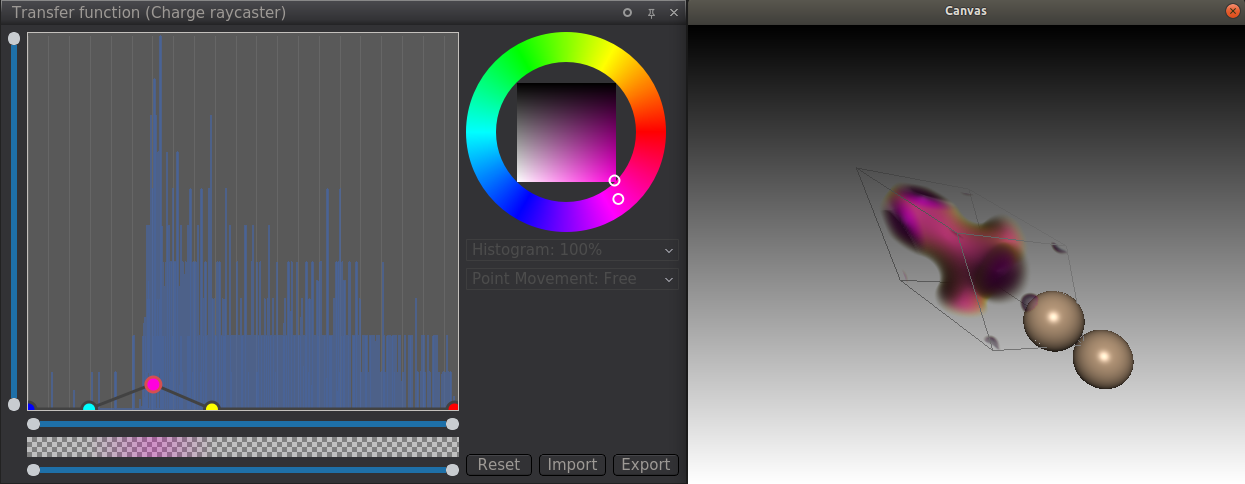
\includegraphics[scale=0.4]{screenshot_transfer_function_transparent.png}
\caption{Laddningstäthetsvärden mellan 0.15 och 0.45 markeras med en någorlunda genomskinlig lila yta.}
\label{fig:transfer_function_transparent}
\end{figure}

\begin{figure} [H]
\centering
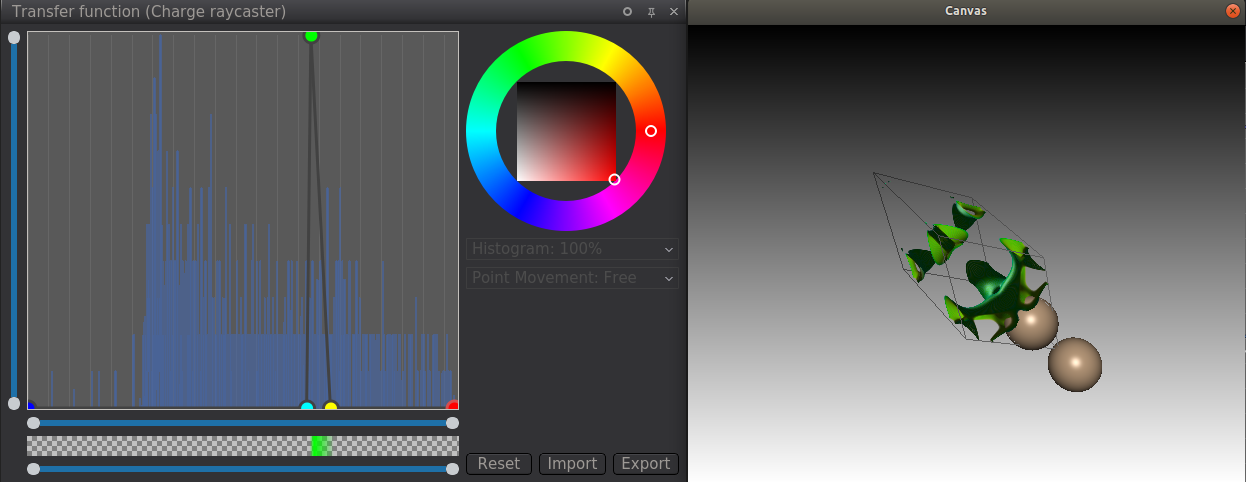
\includegraphics[scale=0.4]{screenshot_transfer_function_almostiso.png}
\caption{Laddningstäthetsvärden kring 0.7 markeras med en opak grön yta, nästan en isoyta.}
\label{fig:transfer_function_iso}
\end{figure}

Slice-funktioners plans färg och transparens kan även de ändras. Detta i processorn \textit{Volume Slice}, i propertyn \textit{Transfer function}.

% TODO: Lägg till Fermi-ytors färginställning (ej transparens då det är isoytor) om vi behandlar dem.
\end{itemize}

\subsection{Datastrukturer}
Två datastrukturer, Point och Function, har introducerats. Dessa används i vissa av de implementerade processorerna.
\subsubsection{Point}
Denna datatyp representerar en reell 1D-punkt och inkapslar punktens värde (ett flyttal) samt variabel metadata.
\subsubsection{Function}
Denna datatyp representerar en reellvärd funktion av en reell variabel och inkapslar sampelvärden och variabel-metadata för x- och y-axlarna.

\subsection{Processorer}
\label{ch:processorer}
Ett antal processorer har implementerats, dessa kategoriseras och beskrivs nedan.

\subsubsection{Kristallstruktur}
\label{ch:kristallstruktur-processorer}
Nedanstående processorer är relaterade till visualiseringen av kristallstrukturer.

\textbf{\textit{CoordinateReader}} \newline
Från en HDF5-fil läser denna processor koordinater för atompositioner. En sökväg till ett dataset sätts via en property kallad StringProperty. Denna StringProperty ska ha storleken $n*3$ och bestå av 32-bitars flyttal. Utdata från CoordinateReader är $n$ stycken vec3.

Inport:
\begin{itemize}
\item Hdf5::Inport inport\_
\end{itemize}

Utport:
\begin{itemize}
\item DataOutport< std::vector<vec3> > outport\_
\end{itemize}

Properties:
\begin{itemize}
\item StringProperty path\_
\end{itemize}

\textbf{\textit{StructureMesh}} \newline
Atompostionsdata kopplas ihop med rätt atomfärg och radie med StructureMesh-processorn. Dessutom hanterar processorn ''picking''-funktionen som gör det möjligt för användaren att välja atomer genom att klicka på dem. StructureMesh har en multiinport, dit en eller flera CoordinateReader-processorer kan kopplas in. Indata för StructureMesh är atompositionsdata i form av vec3 för varje atomslag. Till denna indata läggs properties för färg, radie och antal till för varje atomslag/processor som kopplas in. Den ger en mesh, som har buffrar för position, färg och radie.

Om picking-funktionen är påslagen får meshen även en pickingbuffer, som innehåller de globala picking id som tilldelas av PickingMappern. Då användaren vänsterklickar på en atom läggs dess lokala id i IntVectorPropertyn. Färgen ändras på alla valda atomer genom att alfalagret sätts till 0,5.

Inport:
\begin{itemize}
\item DataInport< std::vector<vec3>, 0> structure\_
\end{itemize}

Utport:
\begin{itemize}
\item MeshOutport mesh\_
\end{itemize}

Properties:
\begin{itemize}
\item FloatProperty scalingFactor\_
\item FloatMat3Property basis\_
\item BoolProperty fullMesh\_
\item IntProperty timestep\_
\item std::vector< std::unique\_ptr<FloatVec4Property> > colors\_: vektor som innehåller färgproperty för varje atomslag
\item std::vector< std::unique\_ptr<FloatProperty > > radii\_: vektor som innehåller radieproperty för varje atomslag
\item std::vector< std::unique\_ptr<IntProperty> > num\_: vektor som innehåller antalet atomer per tidssteg för varje atomslag
\item BoolProperty enablePicking\_: sann då picking-funktionen är påslagen 
\item IntVectorProperty inds\_: vektor med index på valda atomer
\end{itemize}

\subsubsection{HDF5}
\label{ch:hdf5-processorer}
Nedanstående processorer är ämnade att fungera väl med de HDF5-relaterade processorer som är inkluderade i Inviwo.

\textbf{\textit{HDF5PathSelection*}} \newline
Detta är en grupp av processorer som har funktionalitet liknande den inbyggda processorn HDF5PathSelection. En eller flera av dessa processorer placeras med fördel mellan en HDFSource och en eller flera HDF5To*.

Gemensamt för dessa processorer är  att de på inporten tar en Hdf5-grupp och på utporten skriver noll eller flera av dessa omedelbara undergrupper.

Nedan beskrivs de olika processorerna i denna grupp.

\textbf{HDFpathSelectionInt} \newline
Denna processor väljer en HDF5-grupp med heltalsnamn, baserat på värdet på processorns intProperty\_, eventuellt utökat med ledande nollor till bredden specificerat på processorns zeroPadWidthProperty\_.

HDF5PathSelectionInt kan med fördel användas tillsammans med en OrdinalPropertyAnimator för att plocka ut relevant data ur en HDF5-fil.

Anledningen till att utdata ges som en vektor av HDF5-grupper, trots att processorn alltid skriver exakt en grupp på utporten, är att processorn ska följa samma mönster som, och fungera väl med, resterande processorer.

Inport:
\begin{itemize}
\item DataInport<hdf5::Handle> hdf5HandleInport\_
\end{itemize}

Utport:
\begin{itemize}
\item DataOutport< std::vector<hdf5::Handle> > hdf5HandleVectorOutport\_
\end{itemize}

Properties:
\begin{itemize}
\item IntProperty intProperty\_
\item IntSizeTProperty zeroPadWidthProperty\_
\end{itemize}

\textbf{HDF5PathSelectionIntVector} \newline
Denna processor väljer noll eller flera HDF5-grupper med heltalsnamn, baserat på värdet på processorns intVectorProperty\_, eventuellt utökat med ledande nollor till berdden specificerat av processorns zeroPadWidthProperty\_. 

HDF5PathSelectionIntVector kan med fördel användas tillsammans med ''picking'' för att plocka ut relevant data ur en HDF5-fil.

Inport:
\begin{itemize}
\item DataInport<hdf5::Handle> hdf5HandleInport\_
\end{itemize}

Utport:
\begin{itemize}
\item DataOutport< std::vector<hdf5::Handle> > hdf5HandleVectorOutport\_
\end{itemize}

Properties:
\begin{itemize}
\item IntVectorProperty intVectorProperty\_
\item IntSizeTProperty zeroPadWidthProperty\_
\end{itemize}

\textbf{HDF5PathSelectionAllChildren}\newline
Denna processor väljer den givna HDF5-gruppens alla undergrupper.

Inport:
\begin{itemize}
\item DataInport<hdf5::Handle> hdf5HandleInport\_
\end{itemize}

\textbf{\textit{HDF5To*}}\newline
Detta är en grupp av processorer som har funktionalitet liknande den inbyggda processorn HDF5ToVolume. Processorerna placeras med fördel efter en HDFSource-processor, med en eller flera mellan liggande HDF5PathSelection*.

Gemensamt för dessa är att de som indata tar noll eller flera HDF5-grupper (baserat på *pathSelectionProperty\_), plockar ut dataset för varje grupp och omvandlar dessa till relevanta objekt (Point eller Function) som sedan skrivs till utporten. Objektens variabel-metadata tas, om de finns tillgängliga, från attributen associerade med dataseten. Vidare kan, om så väljs med *namePrependParentsProperty\_, metadat utökas med namnen på de grupper var i dataseten ligger.

Vilka dataset som kan väljas med *pathSelectionProperty\_ uppdateras dynamiskt beroende på vilka grupper som ligger på inporten. När ett lämpligt dataset valts kan *pathFreezeProperty\_ användas för att stänga av denna dynamik, så att värdet sparas även om grupperna på inporten (antagligen tillfälligt) ändras. Detta underlättar manuellt experimenterande samt användandet av processorer som tillfälligt ger noll grupper som utadat, t.ex. HDF5PathSelectionIntVector.

\textbf{HDF5ToPoint} \newline
Denna processor konverterar HDF5-data till noll eller flera Point-objekt.

Inport:
\begin{itemize}
\item DataInport<hdf5::Handle, 0, true> hdf5HandleFlatMultiInport\_
\end{itemize}

Utport:
\begin{itemize}
\item DataOutport< std::vector<Point> > pointVectorOutport\_
\end{itemize}

Properties:
\begin{itemize}
\item OptionPropertyString pathSelectionProperty\_
\item BoolProperty pathFreezeProperty\_
\item IntSizeTProperty namePrependParentsProperty
\end{itemize}

\textbf{HDF5ToFunction}\newline
Denna processor konverterar HDF5-data till noll eller flera Function-objekt. 

Normalt plockas två dataset per grupp ut, ett för x-axeln och ett för y-axeln. Om endast data för y-axeln finns tillgänglig kan implicitXProperty\_ sättas, varvid processorn automatgenererar data för x-axeln.

Inport:
\begin{itemize}
\item DataInport<hdf5::Handle, 0, true> hdf5HandleFlatMultiInport\_
\end{itemize}

Utport:
\begin{itemize}
\item DataOutport< std::vector<Function> > functionVectorOutport\_
\end{itemize}

Properties:
\begin{itemize}
\item BoolProperty implicitXProperty\_
\item OptionPropertyString xPathSelectionProperty\_
\item OptionPropertyString yPathSelectionProperty\_
\item BoolProperty xPathFreezeProperty\_
\item BoolProperty yPathFreezeProperty\_
\item IntSizeTProperty xNamePrependParentsProperty\_
\item IntSizeTProperty yNamePrependParentsProperty\_
\end{itemize}

\subsubsection{2D}
\label{ch:2d-processorer}
Nedanstående processorer är ämnade att bearbeta och presentera 2D-data, närmare bestämt data av typen Point och Function.

\textbf{\textit{FunctionOperationUnary}}\newline
Denna processor implementerar en unär operator, antingen negation $(g_{i}(x) = -f_{i}(x))$ eller (multiplikativ) inversion $(g_{i}(x) = 1/f_{i}(x))$. Operatorn appliceras på funktioner på inporten, en i taget, och skriver respektive resultat på utporten.

Inport:
\begin{itemize}
\item DataFrameInport dataframeInport\_
\end{itemize}

Utport:
\begin{itemize}
\item DataFramOutport dataframOutport\_
\end{itemize}

Properties:
\begin{itemize}
\item OptionPropertyString operationProperty\_
\end{itemize}

\textbf{\textit{FunctionOperationNary}}\newline
Denna processor implementerar en operator med variabel aritet (engelska n-ary), antingen addition/summa $(g(x) = \Sigma_{i}f_{i}(x))$ eller multiplikation/produkt $(g(x) = \Pi_{i}f_{i}(x))$. Operatorn appliceras på samtliga funktioner på inporten och skrver resultatet på utporten.

Då funktionerna på inporten kan vara samplade vid olika x-värden behöver processorn ta beslut om var ut-funktionen ska samplas. Processorn utgår från att sampla i samtliga x-värden för samtliga in-funktioner. sampleFilterEnableProperty\_ kan sättas för att filtrera dessa. Då sampleFilterEnableProperty\_ är satt ser processorn till att sampelavståndet är minst det värde som anges i sampleFilterEpsilonProperty\_. När processorn skapas är sampleFilterEnableProperty\_ satt och sampleFilterEpsilonProperty\_ är 0 vilket innebär att x-värden som är identiska filtreras bort.

Om ett värde behöver beräknas vid ett x-värde där en in-funktion inte är samplat används linjär interpolation om x-värdet ligger innanför funktionens definitionsintervall. Om x-värdet ligger utanför detta intervall används undefinedFallbackProperty\_ för att avgöra vilket värde som används istället. Detta kan antingen vara noll eller funktionens värde vid intervallets relevanta ändpunkt.

Inport
\begin{itemize}
\item org.envision.FunctionFlatMultiInport functionFlatMultiInport\_ 
\end{itemize}

Utport:
\begin{itemize}
\item DataFramOutport dataframOutport\_
\end{itemize}

Properties:
\begin{itemize}
\item OptionsPropertyString operationProperty\_
\item OptionsPropertyString undefinedFallbackProperty\_
\item BoolProperty sampleFilterEnableProperty\_
\item FloatProperty sampleFilterEpsilonProperty\_
\end{itemize}

\textbf{\textit{lineplotprocessor}}\newline
lineplotprocessor tar en \emph{DataFrame} som förväntas innehålla två
kolumner med punkter, kallade X och Y. Den konstruerar en mesh som
representerar en linjegraf och denna mesh renderas sedan förslagsvis
med hjälp av en \emph{2D Mesh Renderer}-processor för att generera en
bild av grafen.

lineplotprocessor genererar även en utbild att lägga över grafen som
innehåller axelgraderingen. Axelgraderingen kan också den skickas in i
\emph{2D Mesh Renderer}-processorn och kommer då läggas ovanpå grafen.

Inställningar som har \emph{range} i namnet justerar minimum- och
maximumvärden på koordinataxlarna. Inställningar med \emph{width}
eller \emph{colour} justerar bredd respektive färg för olika linjer
ritade i diagrammet.

\emph{label\_number\_} anger antalet divisioner på koordinataxlarna. Är
värdet till exempel satt till tjugo innebär det att varje axel kommer
ha tjugo divisioner och tjugo axelgraderingsetiketter.

\emph{font\_} ställer in vilket typsnitt axelgraderingen skall ha.

\emph{enable\_line\_} aktiverar ritandet av en vertikal linje på
x-koordinaten specificerad i \emph{line\_x\_coordinate\_}. Denna är
avsedd att ge en visuell markering av var specifika x-värden finns på
x-axeln.

Inport:
\begin{itemize}
    \item DataFrameInport dataFrameInport\_
\end{itemize}

Utports:
\begin{itemize}
    \item MeshOutport meshOutport\_
    \item ImageOutport labels\_
\end{itemize}

Properties:
\begin{itemize}
    \item FloatVec4Property colour\_
    \item FloatVec2Property x\_range\_
    \item FloatVec2Property y\_range\_
    \item FloatProperty scale\_
    \item BoolProperty enable\_line\_
    \item FloatProperty line\_x\_coordinate\_
    \item FloatVec4Property line\_colour\_
    \item FloatVec4Property axis\_colour\_
    \item FloatProperty axis\_width\_
    \item FloatVec4Property grid\_colour\_
    \item FloatProperty grid\_width\_
    \item FontProperty font\_
    \item FloatVec4Property text\_colour\_
    \item IntProperty label\_number\_
\end{itemize}


\subsection{Properties och widgets}

\subsubsection{IntVectorpropety}
Denna property består av en vektor av int-värden.
\subsubsection{IntVectorPropertyWidget}
En widget för IntVectorProperty. ''Textbox'', satt till endast läsning (read only), som innehåller de värden som finns i tillhörande IntVectorProperty.

\section{Utvecklingsmöjligheter}
De egenskaper som visualiserats under 2018 års projekt kan fortfarande vidareutvecklas för att få nya funktioner eller för att presentera datan på ett annat sätt om det anses mer lättförståeligt eller givande.

Molekyldynamik och bandstruktur är två egenskaper som inte har behandlats under detta års projektarbete men som det finns möjlighet att uppdatera från 2017 års projektarbete. I StructureMesh-processorn kan en property läggas till som möjliggör molekyldynamik. För bandstrukturvisualisering finns en parser och samt en visualiseringsmodul som kräver uppdatering.

Detta år har Fermi-ytor varit en av egenskaperna som skulle visualiseras, det hann dock inte bli helt klart. Mycket arbete har ändå lagts ner som det finns möjlighet att bygga vidare på och få att fungera. 

\newpage
\addcontentsline{toc}{section}{Referenser}
\printbibliography{}

\begin{appendices}

\section{HDF5-datastruktur}
\label{appendix:hdf5-format}
\begin{figure}[H]
    \centering
    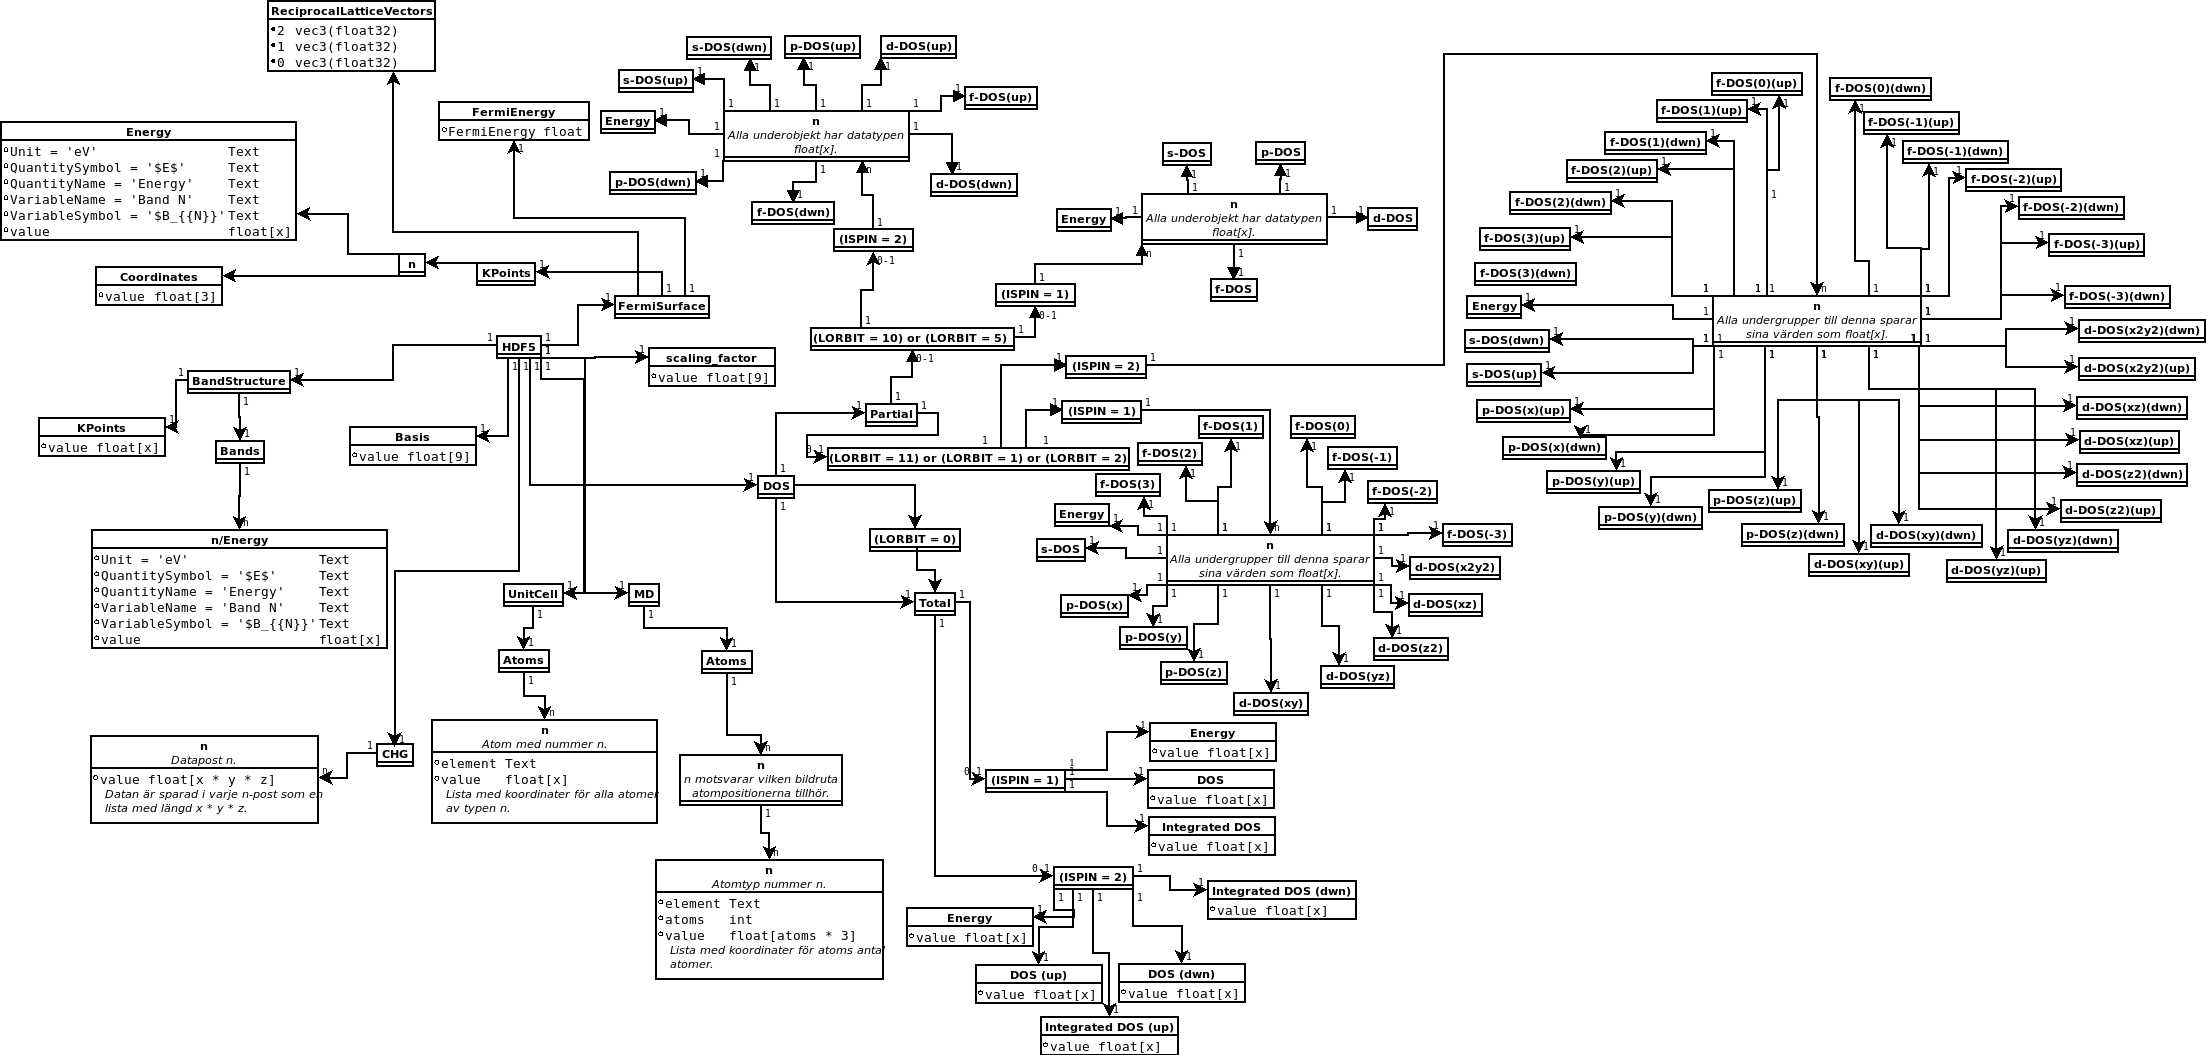
\includegraphics[scale=0.28,angle=-90,origin=c]{hdf5-dataformat3.png}
    \caption{Dataformatet som används när VASP konverteras till HDF5.}
    \label{fig:hdf5-dataformat-roterad}
\end{figure}

\section{HDF5-datastruktur i två delar}
\label{appendix:hdf5-format2}
\begin{figure}[H]
    \centering
    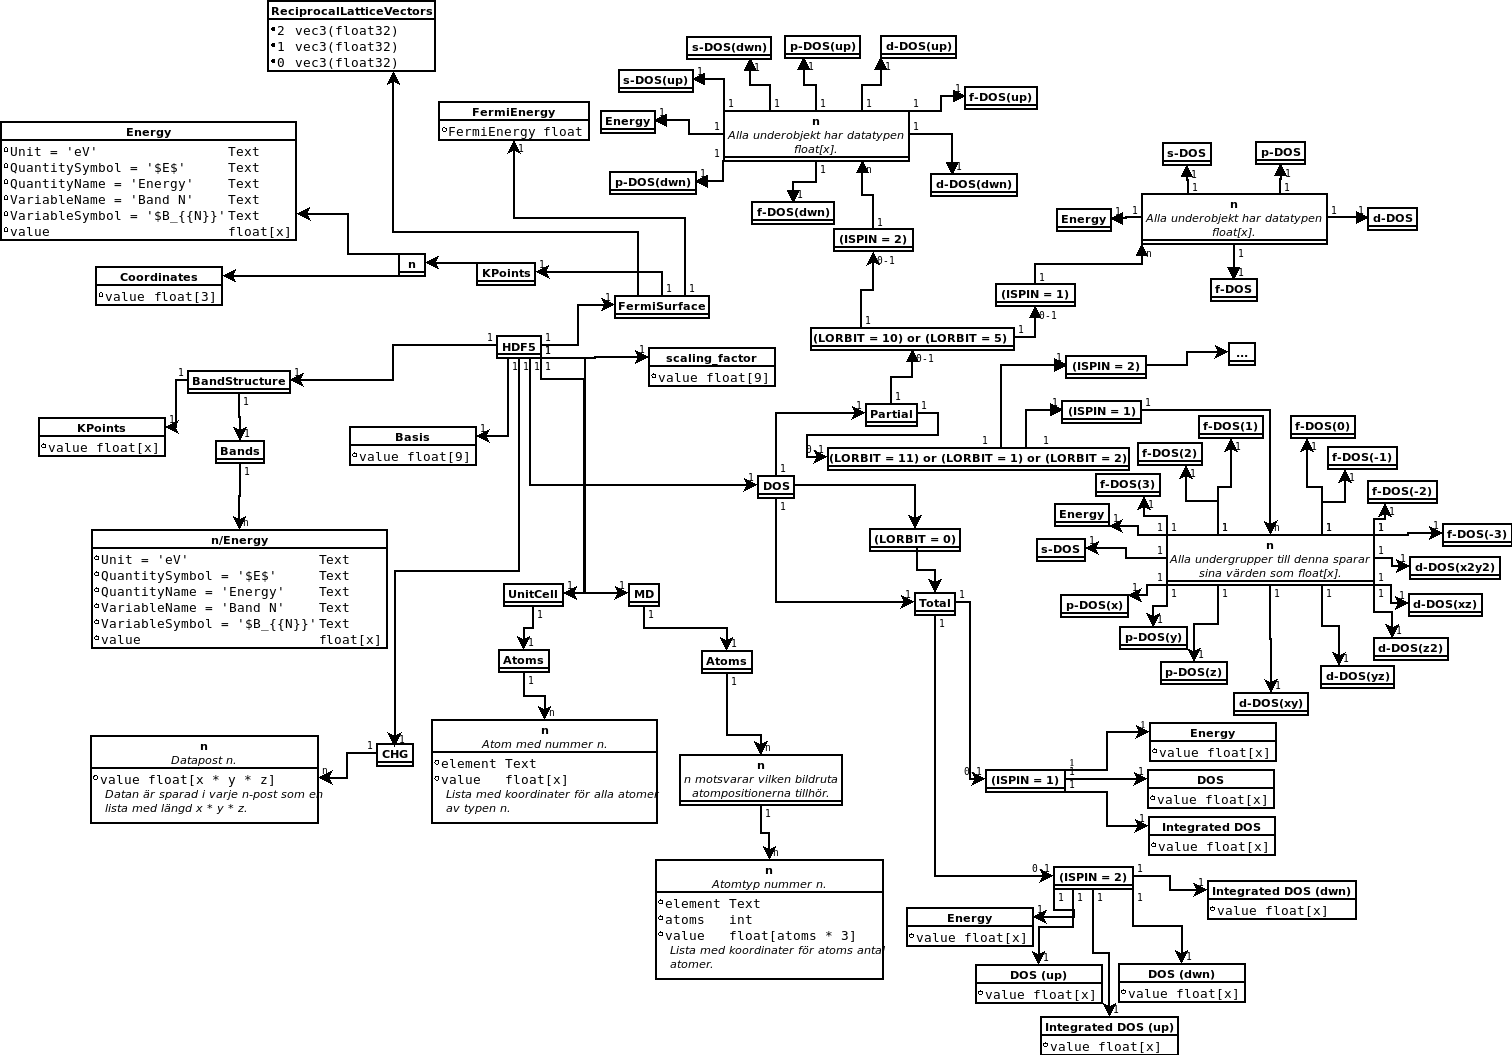
\includegraphics[scale=0.42,angle=-90,origin=c]{hdf5-dataformat3del1.png}
    \caption{Dataformatet som används när VASP konverteras till HDF5 del 1.}
\end{figure}

\begin{figure}[H]
    \centering
    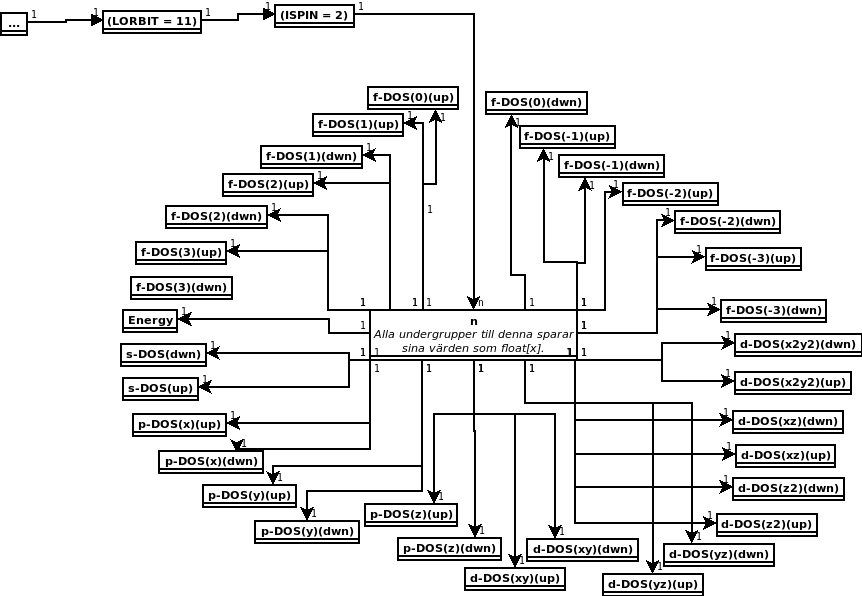
\includegraphics[scale=0.50,angle=-90,origin=c]{hdf5-dataformat3del2.png}
    \caption{Dataformatet som används när VASP konverteras till HDF5 del 2.}
\end{figure}



\newpage
\section{Licens}
\label{ref:licens}
 Creative Commons Legal Code

CC0 1.0 Universal

    CREATIVE COMMONS CORPORATION IS NOT A LAW FIRM AND DOES NOT PROVIDE
    LEGAL SERVICES. DISTRIBUTION OF THIS DOCUMENT DOES NOT CREATE AN
    ATTORNEY-CLIENT RELATIONSHIP. CREATIVE COMMONS PROVIDES THIS
    INFORMATION ON AN ``AS-IS'' BASIS. CREATIVE COMMONS MAKES NO WARRANTIES
    REGARDING THE USE OF THIS DOCUMENT OR THE INFORMATION OR WORKS
    PROVIDED HEREUNDER, AND DISCLAIMS LIABILITY FOR DAMAGES RESULTING FROM
    THE USE OF THIS DOCUMENT OR THE INFORMATION OR WORKS PROVIDED
    HEREUNDER.

Statement of Purpose

The laws of most jurisdictions throughout the world automatically confer
exclusive Copyright and Related Rights (defined below) upon the creator
and subsequent owner(s) (each and all, an ``owner'') of an original work of
authorship and/or a database (each, a ``Work'').

Certain owners wish to permanently relinquish those rights to a Work for
the purpose of contributing to a commons of creative, cultural and
scientific works ("Commons") that the public can reliably and without fear
of later claims of infringement build upon, modify, incorporate in other
works, reuse and redistribute as freely as possible in any form whatsoever
and for any purposes, including without limitation commercial purposes.
These owners may contribute to the Commons to promote the ideal of a free
culture and the further production of creative, cultural and scientific
works, or to gain reputation or greater distribution for their Work in
part through the use and efforts of others.

For these and/or other purposes and motivations, and without any
expectation of additional consideration or compensation, the person
associating CC0 with a Work (the "Affirmer"), to the extent that he or she
is an owner of Copyright and Related Rights in the Work, voluntarily
elects to apply CC0 to the Work and publicly distribute the Work under its
terms, with knowledge of his or her Copyright and Related Rights in the
Work and the meaning and intended legal effect of CC0 on those rights.

1. Copyright and Related Rights. A Work made available under CC0 may be
protected by copyright and related or neighboring rights ("Copyright and
Related Rights"). Copyright and Related Rights include, but are not
limited to, the following:

  i. the right to reproduce, adapt, distribute, perform, display,
     communicate, and translate a Work;
     
 ii. moral rights retained by the original author(s) and/or performer(s);
 
iii. publicity and privacy rights pertaining to a person's image or
     likeness depicted in a Work;
     
 iv. rights protecting against unfair competition in regards to a Work,
     subject to the limitations in paragraph 4(a), below;
     
  v. rights protecting the extraction, dissemination, use and reuse of data in a Work;
  
 vi. database rights (such as those arising under Directive 96/9/EC of the
     European Parliament and of the Council of 11 March 1996 on the legal
     protection of databases, and under any national implementation
     thereof, including any amended or successor version of such
     directive); and
     
vii. other similar, equivalent or corresponding rights throughout the
     world based on applicable law or treaty, and any national
     implementations thereof.

2. Waiver. To the greatest extent permitted by, but not in contravention
of, applicable law, Affirmer hereby overtly, fully, permanently,
irrevocably and unconditionally waives, abandons, and surrenders all of
Affirmer's Copyright and Related Rights and associated claims and causes
of action, whether now known or unknown (including existing as well as
future claims and causes of action), in the Work (i) in all territories
worldwide, (ii) for the maximum duration provided by applicable law or
treaty (including future time extensions), (iii) in any current or future
medium and for any number of copies, and (iv) for any purpose whatsoever,
including without limitation commercial, advertising or promotional
purposes (the "Waiver"). Affirmer makes the Waiver for the benefit of each
member of the public at large and to the detriment of Affirmer's heirs and
successors, fully intending that such Waiver shall not be subject to
revocation, rescission, cancellation, termination, or any other legal or
equitable action to disrupt the quiet enjoyment of the Work by the public
as contemplated by Affirmer's express Statement of Purpose.

3. Public License Fallback. Should any part of the Waiver for any reason
be judged legally invalid or ineffective under applicable law, then the
Waiver shall be preserved to the maximum extent permitted taking into
account Affirmer's express Statement of Purpose. In addition, to the
extent the Waiver is so judged Affirmer hereby grants to each affected
person a royalty-free, non transferable, non sublicensable, non exclusive,
irrevocable and unconditional license to exercise Affirmer's Copyright and
Related Rights in the Work (i) in all territories worldwide, (ii) for the
maximum duration provided by applicable law or treaty (including future
time extensions), (iii) in any current or future medium and for any number
of copies, and (iv) for any purpose whatsoever, including without
limitation commercial, advertising or promotional purposes (the
"License"). The License shall be deemed effective as of the date CC0 was
applied by Affirmer to the Work. Should any part of the License for any
reason be judged legally invalid or ineffective under applicable law, such
partial invalidity or ineffectiveness shall not invalidate the remainder
of the License, and in such case Affirmer hereby affirms that he or she
will not (i) exercise any of his or her remaining Copyright and Related
Rights in the Work or (ii) assert any associated claims and causes of
action with respect to the Work, in either case contrary to Affirmer's
express Statement of Purpose.

4. Limitations and Disclaimers.

 a. No trademark or patent rights held by Affirmer are waived, abandoned,
    surrendered, licensed or otherwise affected by this document.
    
 b. Affirmer offers the Work as-is and makes no representations or
    warranties of any kind concerning the Work, express, implied,
    statutory or otherwise, including without limitation warranties of
    title, merchantability, fitness for a particular purpose, non
    infringement, or the absence of latent or other defects, accuracy, or
    the present or absence of errors, whether or not discoverable, all to
    the greatest extent permissible under applicable law.
    
 c. Affirmer disclaims responsibility for clearing rights of other persons
    that may apply to the Work or any use thereof, including without
    limitation any person's Copyright and Related Rights in the Work.
    Further, Affirmer disclaims responsibility for obtaining any necessary
    consents, permissions or other rights required for any use of the
    Work.
    
 d. Affirmer understands and acknowledges that Creative Commons is not a
    party to this document and has no duty or obligation with respect to
    this CC0 or use of the Work.
    
 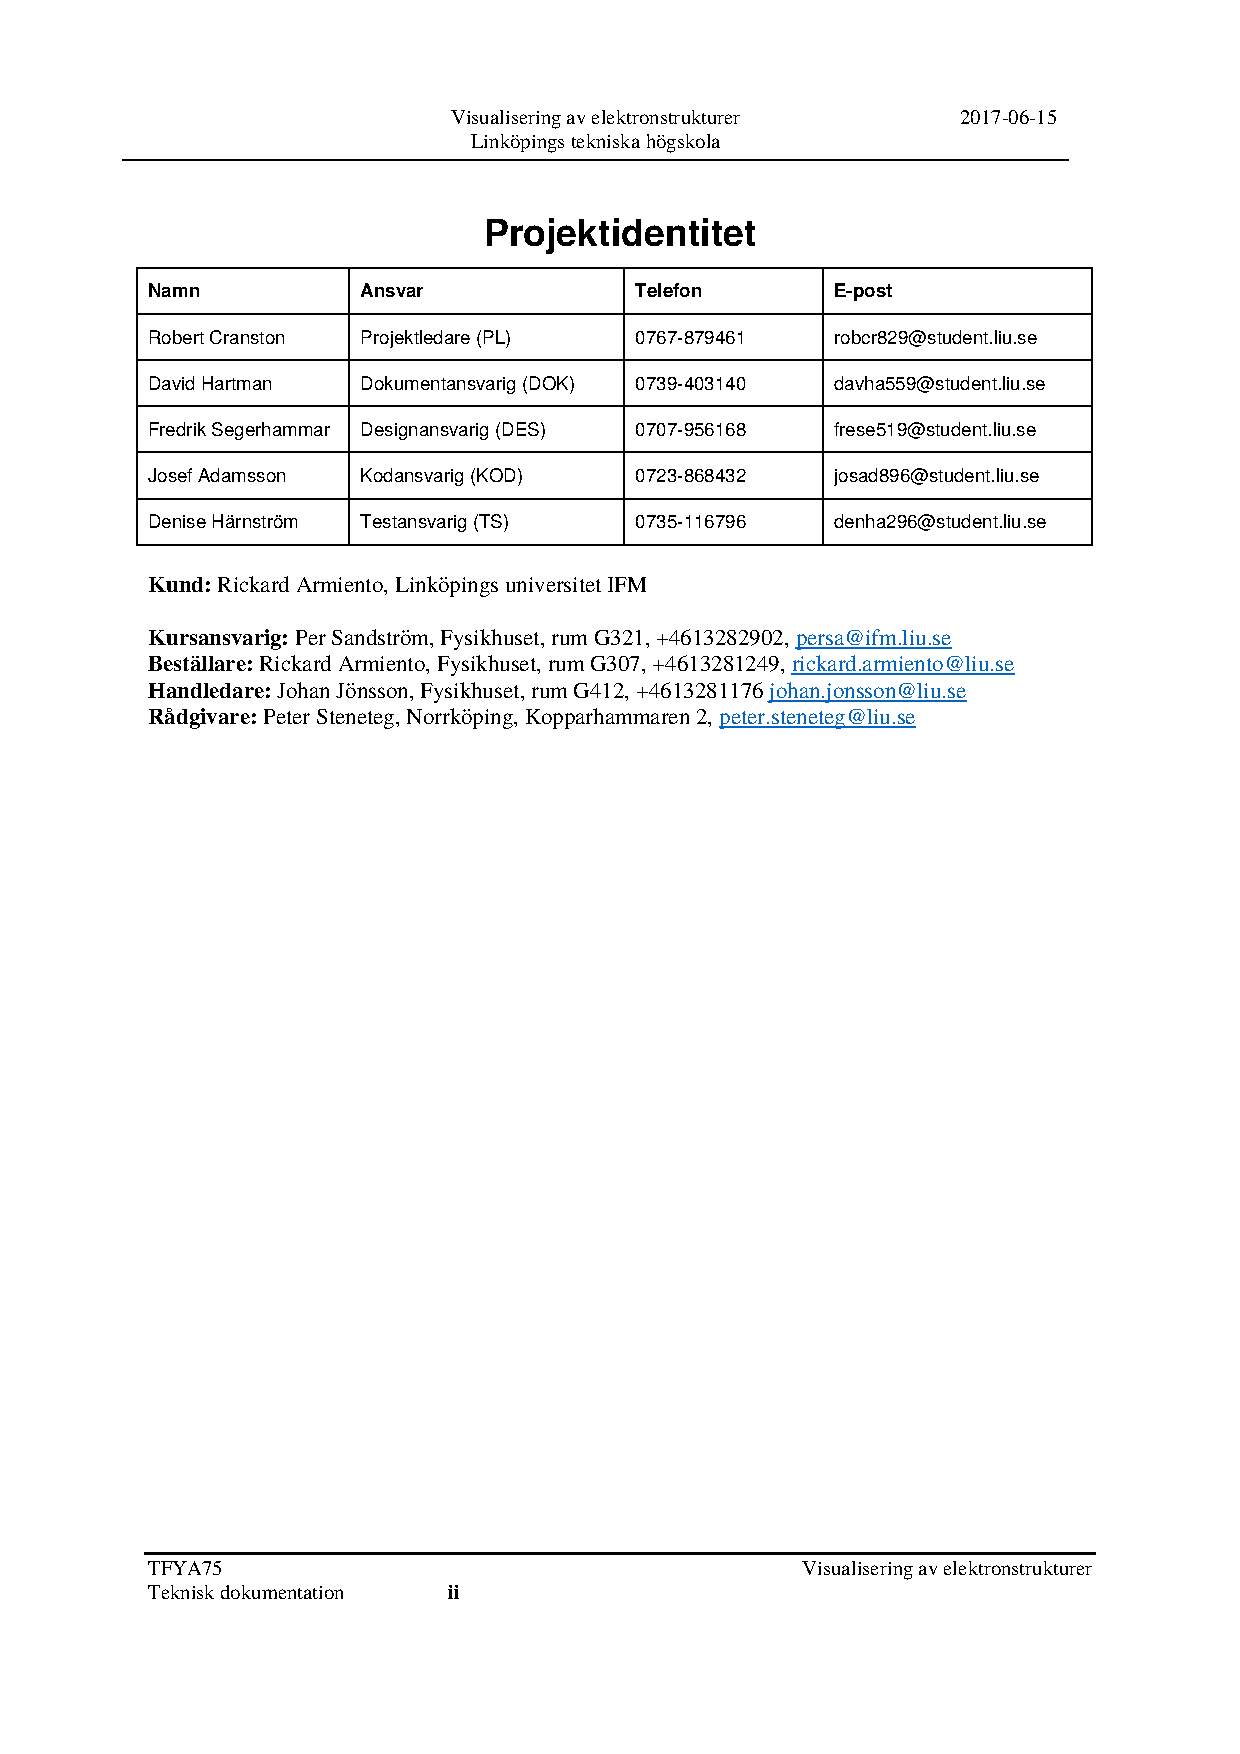
\includepdf[pages={1},offset= 0mm -15mm,pagecommand=\section{Projektgrupp 2017}\label{appendix:tekdok-2017}\thispagestyle{empty}]{2017-authors.pdf}
\includepdf[pages={2-}]{2017-authors.pdf}   
 \end{appendices}
\end{document} 
